\documentclass{article}
\usepackage[T1]{fontenc}
\usepackage{german}  
%%\usepackage[utf8]{inputenc}
\usepackage{graphicx}
\usepackage{xcolor}
\usepackage{ragged2e}
\usepackage{wrapfig}
\usepackage{hyperref}
\usepackage{amssymb}
\usepackage{amsmath}
\usepackage{pgfplots}
\usepackage{enumitem}
\usepackage{color}
\usepackage{mathtools}
\usepackage{mdframed}
\usepackage{makecell}
\usepackage{multirow}
\usepackage{array}
\usepackage[locale=DE]{siunitx}
\usepackage[official]{eurosym}
\usepackage[a4paper,left=1cm,right=1.3cm,top=1.5cm,bottom=2cm,bindingoffset=5mm]{geometry}
\pagenumbering{roman}
\usepackage{titlesec}
\usepackage{tikz}
\usetikzlibrary{3d}
\usetikzlibrary{patterns}
\usetikzlibrary{decorations.markings}
\usepackage[european,straightvoltages]{circuitikz}
\titleformat*{\section}{\large\bfseries}
\setlength{\fboxrule}{0.4mm}
\usepackage{hyperref}

\pgfplotsset{compat=1.17}
\mdfsetup{skipabove=0pt,skipbelow=0pt,linewidth=0.5mm}
\hypersetup{colorlinks=true,urlcolor=blue!70!white}

\title{
    \vspace{-1.5cm}
    \rule{\textwidth}{1.6pt}\vspace*{-\baselineskip}\vspace*{2.1pt}
    \rule{\textwidth}{0.4pt}
    \vspace{0.3\baselineskip}
    
    \textbf{Elektrotechnik I für Wirtschaftsingenieure - Zusammenfassung}
    
    \vspace{0.75\baselineskip}
    \rule{\textwidth}{0.4pt}\vspace*{-\baselineskip}\vspace*{3.2pt}
    \rule{\textwidth}{1.6pt}
    }
\author{J.D.}
\date{September 2021}

\begin{document}
\maketitle


\section{Grundlegendes}
\vspace{-0.8\baselineskip}
\centering
\fbox{\begin{minipage}{\textwidth}
\vspace{0.2\baselineskip}
\centering{\fbox{\textbf{Schaltzeichen}}}\\
\vspace{0.4\baselineskip}
\begin{tabular}{ccccccc}
\ctikzset{bipoles/thickness=1}
\begin{circuitikz}[line width=1pt, scale=0.8, transform shape, voltage shift = 0.5]
\Large
\draw (0,0) to[vsource, v<=$U$] (0,2);
\end{circuitikz} &
\ctikzset{bipoles/thickness=1}
\begin{circuitikz}[line width=1pt, scale=0.8, transform shape, voltage shift = 0.5]
\Large
\draw (0,0) to[isource, l=$I$] (0,2);
\end{circuitikz} &
\raisebox{2\height}{\ctikzset{bipoles/thickness=1}
\begin{circuitikz}[line width=1pt, scale=0.6, transform shape, voltage shift = 0.5]
\Large
\draw (0,0) to[R] (2.5,0);
\end{circuitikz}} &
\raisebox{0.6\height}{\ctikzset{bipoles/thickness=1}
\begin{circuitikz}[line width=1pt, scale=0.7, transform shape, voltage shift = 0.5]
\large
\draw (0,0) to[C] (2,0);
\end{circuitikz}} &
\raisebox{1.6\height}{\ctikzset{bipoles/thickness=1}
\begin{circuitikz}[line width=1pt, scale=0.7, transform shape, voltage shift = 0.5]
\large
\draw (0,0) to[L] (2.5,0);
\end{circuitikz}} &
\raisebox{0.2\height}{\ctikzset{bipoles/thickness=1}
\begin{circuitikz}[line width=1pt, scale=1.8, transform shape, voltage shift = 0.5]
\large
\draw (0,0) node[ground]{};
\end{circuitikz}} &
\ctikzset{bipoles/thickness=1}
\begin{circuitikz}[line width=1pt, scale=0.8, transform shape, voltage shift = 0.5]
\large
\draw (0,0) to[vsourcesin] (0,2);
\end{circuitikz}\\
\makecell{ideale\\Spannungsquelle} & \makecell{ideale\\Stromquelle} & Widerstand & Kondensator & Spule & Masse & Wechselspannung
\end{tabular}
\end{minipage}}
\vspace{0.5\baselineskip}

\fbox{\begin{minipage}{\textwidth}
\vspace{0.2\baselineskip}
\centering{\fbox{\textbf{elementare Physikalische Größen}}}\\
\vspace{0.4\baselineskip}
\begin{tabular}{l|l}
 \textbf{I} Stromstärke [A] & \textit{`Die Menge des in einer bestimmten Zeit durch einen Leiter fließenden Stroms'}\\
 \textbf{U} Spannung [V] & \textit{`Die Kraft auf freie Elektronen und Ursache des elektrischen Stroms' }\\
 \textbf{R} Widerstand [$\Omega$] & \textit{`Die Behinderung des elektrischen Stroms in einem Leiter'}\\
 \\
 \textbf{C} Kapazität [F] & \textit{`Fähigkeit eines Kondensators durch ein elektrisches Feld eine Spannung zu erzeugen'}\\
 \textbf{L} Induktivität [H] & \textit{`Fähigkeit einer Spule durch ein Magnetfeld eine Spannung zu erzeugen'}\\
 \textbf{P} Leistung [W] & \textit{`Die in einer Zeitspanne umgesetzte Energie'}\\
 \textbf{G} Leitwert [S] & \textit{`Der Kehrwert des elektrischen Widerstands'}
\end{tabular}\\
\vspace{0.5\baselineskip}
\rule{\textwidth-30pt}{0.5pt}
\vspace{0.5\baselineskip}\\
\begin{tabular}{ccc}
    \fbox{Ohmsches Gesetz \textbf{$R = \frac{U}{I}$}} & \fbox{Elektrische Leistung $P = U \cdot I$} & \fbox{Leitwert $G = \frac{1}{R}$}
    \end{tabular}
\vspace{0.2\baselineskip}
\end{minipage}}

\section{Schaltungsanalyse}
\vspace{-0.8\baselineskip}
\fbox{\begin{minipage}{\textwidth}
\vspace{0.2\baselineskip}
\centering{\fbox{\textbf{Kirchhoffsche Gleichungen}}}\\
\vspace{0.6\baselineskip}
\begin{flushleft}
\vspace{-.3\baselineskip}
\hspace{.1\baselineskip} 1. Kirchhoffsche Gleichung = \textbf{Knotengleichung}\\
\hspace{1.7\baselineskip}\raisebox{-0.5\height}{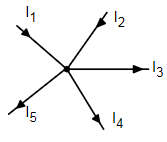
\includegraphics[scale=1.2]{grafiken/knotengleichung.PNG}}
\hspace{1\baselineskip}${I_1 + I_2 - I_3 - I_4 - I_5 = 0}$\hspace{1\baselineskip}
\fbox{\begin{minipage}{0.515\textwidth}
\vspace{1\baselineskip}
\hspace{0.3\baselineskip}${\sum I_k = 0}$\hspace{1\baselineskip}\begin{tabular}{l}
     Vorzeichen + für zufließende Ströme\\
     Vorzeichen $-$ für abfließende Ströme
\end{tabular}
\vspace{1\baselineskip}
\end{minipage}}
\\
\hspace{.1\baselineskip} 2. Kirchhoffsche Gleichung = \textbf{Maschengleichung}\\
\hspace{0.5\baselineskip}\raisebox{-0.5\height}{\ctikzset{bipoles/thickness=1}
\begin{circuitikz}[line width=1pt, scale=0.8, transform shape, voltage shift = 0.5]
\large
\draw (0,2) to[vsource,v_=$U_0$] (0,0);
\draw (0,2) to[R,v^=$U_1$] (2,2) to[R,v^=$U_2$] (2,0) to[R,v^=$U_3$] (0,0);
\draw [thick] (1.4,1) arc (0:160:0.4);
\draw [thick, ->] (1.4,1) arc (360:200:0.4);
\end{circuitikz}}
\hspace{0.1\baselineskip}${-U_0 + U_1 + U_2 + U_3 = 0}$\hspace{0.9\baselineskip}
\fbox{\begin{minipage}{0.515\textwidth}
\vspace{1\baselineskip}
\hspace{0.3\baselineskip}${\sum U_M = 0}$\hspace{1\baselineskip}\begin{tabular}{l}
     Vorzeichen + wenn U in Umlaufrichting\\
     Vorzeichen $-$ wenn U gegen Umlaufrichtung
\end{tabular}
\vspace{1\baselineskip}
\end{minipage}}
\end{flushleft}
\end{minipage}}
\vspace{0.5\baselineskip}

\begin{mdframed}
\vspace{0.2\baselineskip}
\centering{\fbox{\textbf{Reihen- und Parallelschaltung}}}\\
\vspace{0.6\baselineskip}
\begin{minipage}{0.25\textwidth}
\vspace{0.5\baselineskip}
\centering{Reihenschaltung}
\vspace{0.2\baselineskip}
\rule{\textwidth-30pt}{0.5pt}
\begin{align*}
R_{ges} &= R_1 + R_2 \\
I_0 &= I_1 = I_2 \\
U_0 &= U_1 + U_2
\end{align*}
\end{minipage}
\raisebox{-0.5\height}{\ctikzset{bipoles/thickness=1}
\begin{circuitikz}[line width=1pt, scale=0.7, transform shape, voltage shift = 0.5]
\large
\draw (0,0) to[vsource, v<=$U_0$, i=$I_0$] (0,4) -- (2,4) to[R,l_=$R_1$,v^=$U_1$,i_=$I_1$] (2,2) to[R,l_=$R_2$,v^=$U_2$,i_=$I_2$] (2,0) -- (0,0);
\end{circuitikz}}
\hspace{0.2\baselineskip}
\vrule
\hspace{0.2\baselineskip}
\raisebox{-0.5\height}{\ctikzset{bipoles/thickness=1}
\begin{circuitikz}[line width=1pt, scale=0.7, transform shape, voltage shift = 0.5]
\large
\draw (0,0) to[vsource, v<=$U_0$, i=$I_0$] (0,3) to[short,-*] (2,3) to[R,l_=$R_1$,v^=$U_1$,i>_=$I_1$] (2,0) -- (0,0);
\draw (2,3) -- (4,3) to[R,l_=$R_2$,v^=$U_2$,i>_=$I_2$] (4,0) to[short,-*] (2,0);
\end{circuitikz}}
\begin{minipage}{0.25\textwidth}
\vspace{0.5\baselineskip}
\centering{Parallelschaltung}
\vspace{0.2\baselineskip}
\rule{\textwidth-30pt}{0.5pt}
\begin{align*}
R_{ges} &= \frac{R_1 \cdot R_2}{R_1 + R_2} \\
I_0 &= I_1 + I_2 \\
U_0 &= U_1 = U_2
\end{align*}
\vspace{0\baselineskip}\\
Für mehr als zwei parallele Widerstände:
\[\frac{1}{R_{ges}} = \frac{1}{R_1} + \frac{1}{R_2} + ... + \frac{1}{R_n}\]
\hspace{0.2\baselineskip}
\end{minipage}\\
\vspace{0.8\baselineskip}
%Box für Spannungsteiler und Stromteiler
\fbox{\begin{minipage}{0.475\textwidth}
\vspace{0.3\baselineskip}
\begin{center}\fbox{Spannungsteiler}\end{center}
\raisebox{-0.5\height}{\ctikzset{bipoles/thickness=1}
\begin{circuitikz}[line width=1pt, scale=0.6, transform shape]
\Large
\draw (0,4) node[ocirc]{} -- (2,4) to[R,l_=$R_1$] (2,2) to[short,-*](2,2) to[R,l_=$R_2$] (2,0);
\draw (2,2) to[short, -o] (4,2);
\draw (0,0) node[ocirc]{} -- (4,0) node[ocirc]{};
\draw (0,4) to[open, v=$U_1$] (0,0);
\draw (4,2) to[open, v=$U_2$] (4,0);
\end{circuitikz}}
\hspace{0.8\baselineskip}
\scalebox{0.92}{\begin{minipage}{0.3\textwidth}\[\frac{U_2}{U_1} = \frac{R_2 \cdot I}{(R_1 + R_2) \cdot I} = \frac{R_2}{R_1 + R_2}\]\end{minipage}}\\
\scalebox{0.98}{\begin{minipage}{\textwidth}\[\small\frac{\text{Teilspannung}}{\text{Gesamtspannung}} = \frac{\text{Widerstand unter Teilspannungsabfall}}{\text{Gesamtwiderstand}}\]\end{minipage}}
\end{minipage}}%
\hspace{0.1\baselineskip}
\fbox{\begin{minipage}{0.475\textwidth}
\vspace{0.3\baselineskip}
\begin{center}\fbox{Stromteiler}\end{center}
\hspace{1.2\baselineskip}
\raisebox{-0.5\height}{\ctikzset{bipoles/thickness=1}
\begin{circuitikz}[line width=1pt, scale=0.6, transform shape, voltage shift = 0.5]
\Large
\draw (0,3) to[short,-*,i=$I_0$] (2,3) to[R,l_=$R_1$,i>_=$I_1$] (2,0) -- (0,0);
\draw (2,3) -- (4,3) to[R,l_=$R_2$,i>_=$I_2$] (4,0) to[short,-*] (2,0);
\end{circuitikz}}
\hspace{1\baselineskip}
\begin{minipage}{0.3\textwidth}\[\frac{I_1}{I_0} = \frac{R_1||R_2}{R_1} = \frac{R_2}{R_1 + R_2}\]\end{minipage}
\vspace{0.7\baselineskip}\\
\vspace{0.1\baselineskip}
\scalebox{0.96}{\begin{minipage}{\textwidth}\[\small\frac{\text{Teilstrom}}{\text{Gesamtstrom}} = \frac{\text{Gesamtwiderstand}}{\text{Vom Teilstrom durchflossener Widerstand}}\]\end{minipage}}
\end{minipage}}

\vspace{0.5\baselineskip}
\rule{0.6\textwidth}{0.5pt}
\begin{minipage}{0.8\textwidth}
\vspace{0.5\baselineskip}
\textit{\small\ Das Verhalten von Strom und Spannung sowie das Rechnen mit Widerständen in Reihen- und Parallelschaltungen sind essenziell für ein gutes, intuitives Verständis einer Schaltung! Auch die Spannungs- und Stromteiler-Regel ist so wichtig, dass man sie jederzeit griffbereit haben sollte.}
\end{minipage}
\vspace{0.3\baselineskip}
\end{mdframed}
\vspace{0.8\baselineskip}

\begin{mdframed}
\vspace{0.2\baselineskip}
\centering{\fbox{\textbf{Spannungsquelle und Stromquelle}}}
\justify
Eine \textit{ideale} Spannungsquelle, welche immer eine konstante Spannung beibehält, müsste bei kurzschließen einen unendlich großen Strom erzeugen, was natürlich nicht realistisch ist. Eine \textit{reale} Spannungsquelle ähnelt daher einer Spannungsquelle mit in Serie geschaltetem Innenwiderstand $R_i$. Das Gleiche passiert bei der Stromquelle, nur wird hier der Innenwiderstand parallel geschaltet.
\par\centering
\vspace{0.6\baselineskip}
\begin{tabular}{ccccc}
    \raisebox{-0.5\height}{\ctikzset{bipoles/thickness=1}
\begin{circuitikz}[line width=1pt, scale=0.8, transform shape, voltage shift = 0.5]
\Large
\draw (0,0) to[vsource, v<=$U$] (0,2);
\end{circuitikz}} & \raisebox{-0.5\height}{\ctikzset{bipoles/thickness=1}
\begin{circuitikz}[line width=1pt, scale=0.8, transform shape, voltage shift = 0.5]
\Large
\fill [gray!15!white](-1.5,-0.5) rectangle (2,2.5);
\draw (0,0) to[vsource, v<=$U$] (0,2) to[R,l_=$R_i$] (2,2) -- (2.5,2);
\draw (0,0) -- (2.5,0);
\end{circuitikz}} &
    \begin{minipage}{1.5cm}\hspace{1.5cm}\end{minipage}&
    \raisebox{-0.5\height}{\ctikzset{bipoles/thickness=1}
\begin{circuitikz}[line width=1pt, scale=0.8, transform shape, voltage shift = 0.5]
\Large
\draw (0,0) to[isource, l=$I$] (0,2);
\end{circuitikz}} & 
    \raisebox{-0.5\height}{\ctikzset{bipoles/thickness=1}
\begin{circuitikz}[line width=1pt, scale=0.8, transform shape, voltage shift = 0.5]
\Large
\fill [gray!15!white](-1,-0.5) rectangle (2.2,2.5);
\draw (0,0) to[isource, l=$I$] (0,2) to[short,-*] (1.2,2) -- (2.7,2);
\draw (1.2,2) to[R=$R_i$] (1.2,0);
\draw (0,0) to[short,-*] (1.2,0) -- (2.7,0);
\end{circuitikz}}\\\\
    ideale Spannungsquelle & reale Spannungsquelle & & ideale Stromquelle & reale Stromquelle
\end{tabular}\\
\vspace{0.5\baselineskip}
\rule{0.6\textwidth}{0.5pt}\\
\vspace{0.5\baselineskip}
Eine \textbf{Transformation} von realer Spannungsquelle zu realer Stromquelle und vice versa ist simpel:
\begin{minipage}{0.8\textwidth}
\vspace{1\baselineskip}
\centering\raisebox{-0.5\height}{\ctikzset{bipoles/thickness=1}
\begin{circuitikz}[line width=1pt, scale=0.8, transform shape, voltage shift = 0.5]
\Large
\fill [gray!15!white](-1.5,-0.5) rectangle (2,2.5);
\draw (0,0) to[vsource, v<=$U$] (0,2) to[R,l_=$R_i$] (2,2) -- (2.5,2);
\draw (0,0) -- (2.5,0);
\draw (2.5,2) to[R=$R$] (2.5,0);
\end{circuitikz}
\hspace{2\baselineskip}
\raisebox{0.9cm}{\scalebox{3}{$\Longleftrightarrow$}}
\hspace{2\baselineskip}
\ctikzset{bipoles/thickness=1}
\begin{circuitikz}[line width=1pt, scale=0.8, transform shape, voltage shift = 0.5]
\Large
\fill [gray!15!white](-1,-0.5) rectangle (2.2,2.5);
\draw (0,0) to[isource, l=$I$] (0,2) to[short,-*] (1.2,2) -- (2.7,2);
\draw (1.2,2) to[R=$R_i$] (1.2,0);
\draw (0,0) to[short,-*] (1.2,0) -- (2.7,0);
\draw (2.7,2) to[R=$R$] (2.7,0);
\end{circuitikz}}
\end{minipage}\\
\vspace{0.5\baselineskip}
\rule{0.6\textwidth}{0.5pt}\\
\vspace{0.5\baselineskip}
Es werden oft zwei \textbf{Grenzfälle} beim Betrieb von Quellen beobachtet:
\vspace{1\baselineskip}

\begin{tabular}{c|c|c|c}
      & \makecell{\textbf{Leerlauf}\\$R_{Last} = \infty$} & \makecell{\textbf{Kurzschluss}\\$R_{Last} = 0$} & Kennlinie \\\hline
     \makecell{\textbf{Spannungsquelle}\\\\\raisebox{-0.5\height}{\ctikzset{bipoles/thickness=1}
\begin{circuitikz}[line width=1pt, scale=0.6, transform shape, voltage shift = 0.5]
\Large
\fill [gray!15!white](-1.5,-0.5) rectangle (2,2.5);
\draw (0,0) to[vsource, v<=$U_L$] (0,2) to[R,l_=$R_i$] (2,2) -- (2.5,2);
\draw (0,0) -- (2.5,0);
\draw (2.5,2) to[R=$R_{Last}$, i>^=$I_{Last}$] (2.5,0);
\end{circuitikz}}\\\\} & \makecell{$U_{Last} = U_L$\\$I_{Last} = 0$} & \makecell{$U_{Last} = 0$\\$I_{Last} = I_k = \frac{U_L}{R_i}$} &\makecell{\raisebox{-0.5\height}{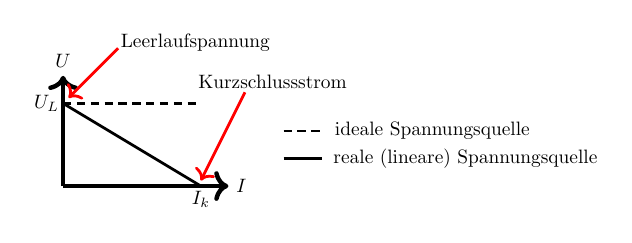
\begin{tikzpicture}[line width=1pt, scale=0.7, transform shape]
\draw [->, ultra thick] (0,0) -- (0,2) node[above]{$U$};
\draw [->, ultra thick] (0,0) -- (3,0) node[right]{$I$};
\draw [densely dashed] (0,1.5) -- (2.5,1.5);
\draw (0,1.5) -- (2.5,0);
\draw [<-, red] (0.1,1.6) -- (1,2.5);
\draw [<-, red] (2.5,0.1) -- (3.3,1.7);
\node [very thick] at (2.4,2.6) {Leerlaufspannung};
\node [very thick] at (3.8,1.9) {Kurzschlussstrom};
\node [] at (2.5, -0.25) {$I_k$};
\node [] at (-0.3,1.5) {$U_L$};

\draw [densely dashed] (4,1) -- (4.7,1);
\node [] at (6.7,1) {ideale Spannungsquelle};
\draw (4,0.5) -- (4.7,0.5);
\node [] at (7.3,0.5) {reale (lineare) Spannungsquelle};
\end{tikzpicture}}\\$U_{Last} = U_L - I_{Last} \cdot R_i$} \\\cline{2-4}
     \makecell{\textbf{Stormquelle}\\\\\raisebox{-0.5\height}{\ctikzset{bipoles/thickness=1}
\begin{circuitikz}[line width=1pt, scale=0.6, transform shape, voltage shift = 0.5]
\Large
\fill [gray!15!white](-1,-0.5) rectangle (2.2,2.5);
\draw (0,0) to[isource, i=$I_k$] (0,2) to[short,-*] (1.2,2) -- (2.7,2);
\draw (1.2,2) to[R=$R_i$] (1.2,0);
\draw (0,0) to[short,-*] (1.2,0) -- (2.7,0);
\draw (2.7,2) to[R=$R_{Last}$, i>^=$I_{Last}$] (2.7,0);
\end{circuitikz}}} & \makecell{$U_{Last} = I_k \cdot R_i$\\$I_{Last} = 0$} & \makecell{$U_{Last} = 0$\\$I_{Last} = I_k = \frac{U_L}{R_i}$} &\makecell{\raisebox{-0.5\height}{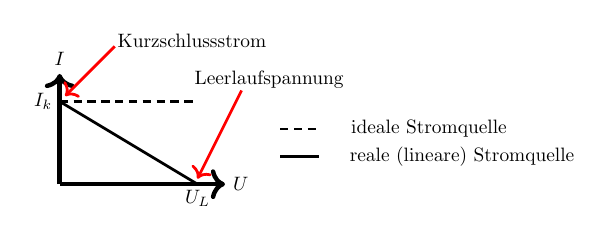
\begin{tikzpicture}[line width=1pt, scale=0.7, transform shape]
\draw [->, ultra thick] (0,0) -- (0,2) node[above]{$I$};
\draw [->, ultra thick] (0,0) -- (3,0) node[right]{$U$};
\draw [densely dashed] (0,1.5) -- (2.5,1.5);
\draw (0,1.5) -- (2.5,0);
\draw [<-, red] (0.1,1.6) -- (1,2.5);
\draw [<-, red] (2.5,0.1) -- (3.3,1.7);
\node [very thick] at (2.4,2.6) {Kurzschlussstrom};
\node [very thick] at (3.8,1.9) {Leerlaufspannung};
\node [] at (2.5, -0.25) {$U_L$};
\node [] at (-0.3,1.5) {$I_k$};

\draw [densely dashed] (4,1) -- (4.7,1);
\node [] at (6.7,1) {ideale Stromquelle};
\draw (4,0.5) -- (4.7,0.5);
\node [] at (7.3,0.5) {reale (lineare) Stromquelle};
\end{tikzpicture}}\\$I_{Last} = I_k - \frac{U_{Last}}{R_i}$}\\\hline
\end{tabular}
\[\text{Innenwiderstand } R_i = \frac{U_L}{I_k} = \frac{\text{Leerlaufspannung}}{\text{Kurzschlussstrom}}\]\\
\end{mdframed}

\flushleft
\section{Kondensator}
\vspace{-0.8\baselineskip}
\begin{mdframed}
\centering
\vspace{0.2\baselineskip}
\centering{\fbox{\textbf{Definition}}}\\
\vspace{0.5\baselineskip}
\raisebox{-0.5\height}{\ctikzset{bipoles/thickness=1}
\begin{circuitikz}[line width=1pt, scale=0.7, transform shape, voltage shift = 0.5]
\large
\draw (0,0) to[C] (2,0);
\end{circuitikz}}
\justify
Der \textbf{Kondensator} ist ein elektrisches Bauelement zum kurzzeitigen Speichern elektrischer Ladung in Form eines elektrischen Feldes. Er besteht aus zwei elektrischen Leitern, die durch ein Dielektrikum (Isolator) voneinander getrennt sind. Einfachste Bauform ist der Plattenkondensator mit zwei parallelen Metallplatten und Luft als Dielektrikum.
\par\centering
\raisebox{-0.5\height}{\ctikzset{bipoles/thickness=1}
\begin{circuitikz}[line width=1.4pt, scale=1.2, transform shape, voltage shift = 0.5]
\large
\draw (0,1) -- (1,1);
\draw (1,0.5) -- (1,1.5);
\draw [black, pattern=crosshatch dots, pattern color=black](1.1,0.5) rectangle (1.4,1.5);
\draw (1.5,0.5) -- (1.5,1.5);
\draw (1.5,1) -- (2.5,1);
\draw [<-, very thick] (1.35,1.6) -- (1.9,1.7); 
\node [] at (2.8,1.7) {\scriptsize Dielektrikum};
\end{circuitikz}}
\raisebox{-0.5\height}{\ctikzset{bipoles/thickness=1}
\begin{circuitikz}[line width=1.2pt, scale=0.7, transform shape, voltage shift = 0.5]
\large
\draw (0,0) to[vsource, v<=$U_0$] (0,3) -- (4,3) -- (4,2.5);
\draw (0,0) -- (4,0) -- (4,0.5);
\draw [black] (2.5,2.1) rectangle (5.5,2.5);
\draw [black] (2.5,0.5) rectangle (5.5,0.9);
\node [] at (3,2.3) {$+$};
\node [] at (3.5,2.3) {$+$};
\node [] at (4,2.3) {$+$};
\node [] at (4.5,2.3) {$+$};
\node [] at (5,2.3) {$+$};
\node [] at (3,0.7) {$-$};
\node [] at (3.5,0.7) {$-$};
\node [] at (4,0.7) {$-$};
\node [] at (4.5,0.7) {$-$};
\node [] at (5,0.7) {$-$};
\draw [->](3,2) -- (3,1);
\draw [->](3.5,2) -- (3.5,1);
\draw [->](4,2) -- (4,1);
\draw [->](4.5,2) -- (4.5,1);
\draw [->](5,2) -- (5,1);
\end{circuitikz}}
\justify
Bei angelegter Spannung herrscht oben ein Elektronendefizit während sich unten die Elektronen häufen. Zwischen den Platten entsteht ein elektrisches Feld. Der Kondensator ist `geladen'. Da die Platten elektrisch nicht miteinander verbunden sind, kann im geladenen Zustand kein Strom fließen. Falls die Spannungsquelle entfernt wird, bleibt die Ladung am Kondensator und damit die Spannung (kurzfristig) erhalten. Sobald der Stromkreis geschlossen wird, beispielsweise durchs anschließen einer LED, fließt Strom und der Kondensator wird `entladen'.
\[\text{Kapazität } C = \frac{Q}{U} \hspace{2cm} \text{für Plattenkondensatoren } C = \varepsilon_0\varepsilon_r\frac{A}{d}\]
\[\text{Elektrische Feldstärke } E = \frac{U}{d}\]
\[\text{Elektrische Energie } W = \frac{1}{2}CU^2\]
\end{mdframed}
\vspace{0.7\baselineskip}

\begin{mdframed}
\centering
\vspace{0.2\baselineskip}
\fbox{\textbf{Reihen- und Parallelschaltung}}\\
\vspace{0.5\baselineskip}
\begin{tabular}{cc}
    &\\
    \makecell{\raisebox{-0.25\height}{\ctikzset{bipoles/thickness=1}
\begin{circuitikz}[line width=1pt, scale=0.7, transform shape, voltage shift = 0.5]
\large
\draw (0,0) to[C,l=$C_1$] (1.5,0) to[C,l=$C_2$] (3,0) to[C,l=$C_3$] (4.5,0);
\end{circuitikz}} \hspace{0.7\baselineskip} \scalebox{1.3}{$\frac{1}{C} = \frac{1}{C_1} + \frac{1}{C_3} + \frac{1}{C_3}$}} & \makecell{\raisebox{-0.4\height}{\ctikzset{bipoles/thickness=1}
\begin{circuitikz}[line width=1pt, scale=0.6, transform shape, voltage shift = 0.5]
\large
\draw (0,2) to[short,-*] (1,2) to[short,-*] (2,2) -- (3,2) to[C,name=C3] (3,0) to[short,-*] (2,0) to[short,-*] (1,0) -- (0,0);
\draw (1,2) to[C,name=C1] (1,0);
\draw (2,2) to[C,name=C2] (2,0);
\node[above, yshift=3pt] at (C1.n) {$C_1$};
\node[above, yshift=3pt] at (C2.n) {$C_2$};
\node[above, yshift=3pt] at (C3.n) {$C_3$};
\end{circuitikz}} \hspace{0.7\baselineskip} $C = C_1 + C_2 + C_3$} \\
    &\\
    Reihenschaltung & Parallelschaltung \\
\end{tabular}
\end{mdframed}
\vspace{0.7\baselineskip}

\begin{mdframed}
\centering
\vspace{0.2\baselineskip}
\fbox{\textbf{Ladevorgänge}}\\
\vspace{0.5\baselineskip}
\raisebox{-0.5\height}{\ctikzset{bipoles/thickness=1}
\begin{circuitikz}[line width=1pt, scale=0.9, transform shape, voltage shift = 0.5]
\large
\draw (0,0) to[vsource, v<=$U_0$] (0,3) to[short,-o] (1,3);
\draw [very thick](1.03,3) -- +(30:0.66);
\node [] at (1.4,3.7) {\text{\small\textbf{Laden}}};
\draw (1.7,3) to[short,o-] (2.6,3) to[short,*-,i=$I$] (5,3);
\draw (2.6,3) to[short,-o] (2.6,2);
\draw [very thick](2.6,1.97) -- +(-60:0.66);
\node [] at (1.8,1.7) {\text{\small\textbf{Entladen}}};
\draw (2.6,1.3) to[short,o-] (2.6,0);
\draw (5,3) -- (5,2.6) to[R,l=$R$] (5,1.5) to[C,l=$C$,v=$U_C$] (5,0);
\draw (0,0) to[short,-*] (2.6,0) -- (5,0);
\end{circuitikz}}\\
\vspace{1\baselineskip}
\begin{mdframed}[linewidth=0.4mm]
\flushleft\textbf{\large Kennlinie}\\
\centering
\raisebox{-0.5\height}{\ctikzset{bipoles/thickness=1}
\begin{circuitikz}[line width=1pt, scale=1, transform shape, voltage shift = 0.5]
\large
\draw [->, very thick] (0,0) -- (0,2) node[above]{$U_C$};
\draw [->, very thick] (0,0) -- (8,0) node[right]{$t$};
\node [] at (-0.5,1.7) {\small $U_0$};
\draw (-0.1,1.7) -- (0.1,1.7);
\draw [blue] (0,0) .. controls (0.4,1) and (0.7,1.65) .. (2.5,1.7);
\draw [densely dashed] (2.5,1.7) -- (2.5,-4.7);
\draw [blue] (2.5,1.7) -- (5,1.7);
\draw [densely dashed] (5,1.7) -- (5,-4.7);
\draw [blue] (5,1.7) .. controls (5.5,0.7) and (5.9,0.05) .. (7.5,0);
\node [] at (1.3,-0.7) {\text{Laden}};
\node [] at (6.3,-0.7) {\text{Entladen}};
\draw [->, very thick] (0,-4.7) -- (0,-1) node[above]{$I$};
\draw [->, very thick] (0,-3) -- (8,-3) node[right]{$t$};
\draw [green!60!black] (0,-1.3) .. controls (0.5,-2.3) and (0.9,-2.95) .. (2.5,-3);
\draw [green!60!black] (2.5,-3) -- (5,-3);
\draw [green!60!black] (5,-4.7) .. controls (5.4,-3.7) and (5.7,-3.05) .. (7.5,-3);
\node [blue] at (2,-5.2) {$U_C(t) = U_0 \cdot (1-e^{-\frac{t}{R \cdot C}})$};
\node [green!40!black] at (1.2,-6.2) {$I(t) = \frac{U}{R} \cdot e^{-\frac{t}{R \cdot C}}$};
\node [blue] at (6.7,-5.2) {$U_C(t) = U_0 \cdot e^{-\frac{t}{R \cdot C}}$};
\node [green!40!black] at (6.6,-6.2) {$I(t) = -\frac{U}{R} \cdot e^{-\frac{t}{R \cdot C}}$};
\end{circuitikz}} 
\begin{minipage}{0.4\textwidth}
Beim Ladevorgang fließt temporär Strom, bis sich die Spannung am Kondensator eingestellt hat, die auch an der Spannungsquelle anliegt. Beim Entladen fließt wieder Strom, nur in entgegengesetzter Richtung, bis der Kondensator entladen ist und die Spannung Null beträgt.\\ Das allgemeine Zeitverhalten von Spannung und Strom eines Kondensators in Abhängigkeit der jeweils anderen Größe ergibt sich durch:\\ \begin{mdframed}[linewidth=0.7mm]
\vspace{-0.8\baselineskip}
\begin{align*}
u_C(t) &= \frac{1}{C} \int i(t)\,dt \\
i_C(t) &= C \frac{du(t)}{dt}
\end{align*}
\end{mdframed}
\vspace{0.4\baselineskip}
\end{minipage}
\end{mdframed}
\vspace{0.5\baselineskip}
\end{mdframed}

\flushleft
\section{Spule}
\vspace{-0.8\baselineskip}
\begin{mdframed}
\centering
\vspace{0.2\baselineskip}
\centering{\fbox{\textbf{Definition}}}\\
\vspace{0.5\baselineskip}
\raisebox{-0.5\height}{\ctikzset{bipoles/thickness=1}
\begin{circuitikz}[line width=1pt, scale=0.7, transform shape, voltage shift = 0.5]
\large
\draw (0,0) to[L] (2.5,0);
\end{circuitikz}}\\
\justify
Die \textbf{Spule} ist ein elektrisches Bauelement, dem ein langer dünner Leiter spiralförmig um einen meist zylindrischen Körper gewickelt wird. Beim Kondensator haben wir gesehen, dass elektrische Energie in einem elektrischen Feld gespeichert wird. Bei der Spule wird diese Energie in einem Magnetfeld gespeichert.\\
\par\centering
\raisebox{-0.5\height}{\ctikzset{bipoles/thickness=1}
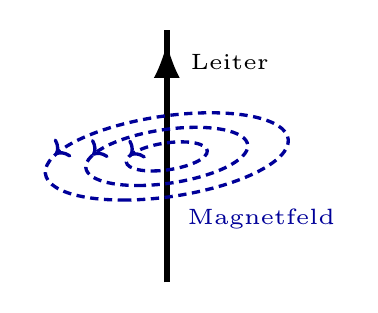
\begin{tikzpicture}[line width=1.2pt, scale=1.6, transform shape, voltage shift = 0.5]
    \begin{scope}[canvas is zy plane at x=0]
     \draw [line width=2pt](0,-1) -- (0,1);
     \draw [-{Latex[scale=1.5]}](0,0) -- (0,0.9);
   \end{scope}

   \begin{scope}[canvas is zx plane at y=0]
     \draw [blue!60!black, densely dashed, decoration={markings, mark=at position 0.8 with {\arrow{>}}}, postaction={decorate}](0,0) circle (0.3cm);
     \draw [blue!60!black, densely dashed, decoration={markings, mark=at position 0.8 with {\arrow{>}}}, postaction={decorate}](0,0) circle (0.6cm);
     \draw [blue!60!black, densely dashed, decoration={markings, mark=at position 0.8 with {\arrow{>}}}, postaction={decorate}](0,0) circle (0.9cm);
   \end{scope}
    
    \node [] at (0.5,0.75) {\text{\tiny Leiter}};
    \node [blue!60!black] at (0.75,-0.5) {\text{\tiny Magnetfeld}};

\end{tikzpicture}}
\hspace{2\baselineskip}
\raisebox{-0.5\height}{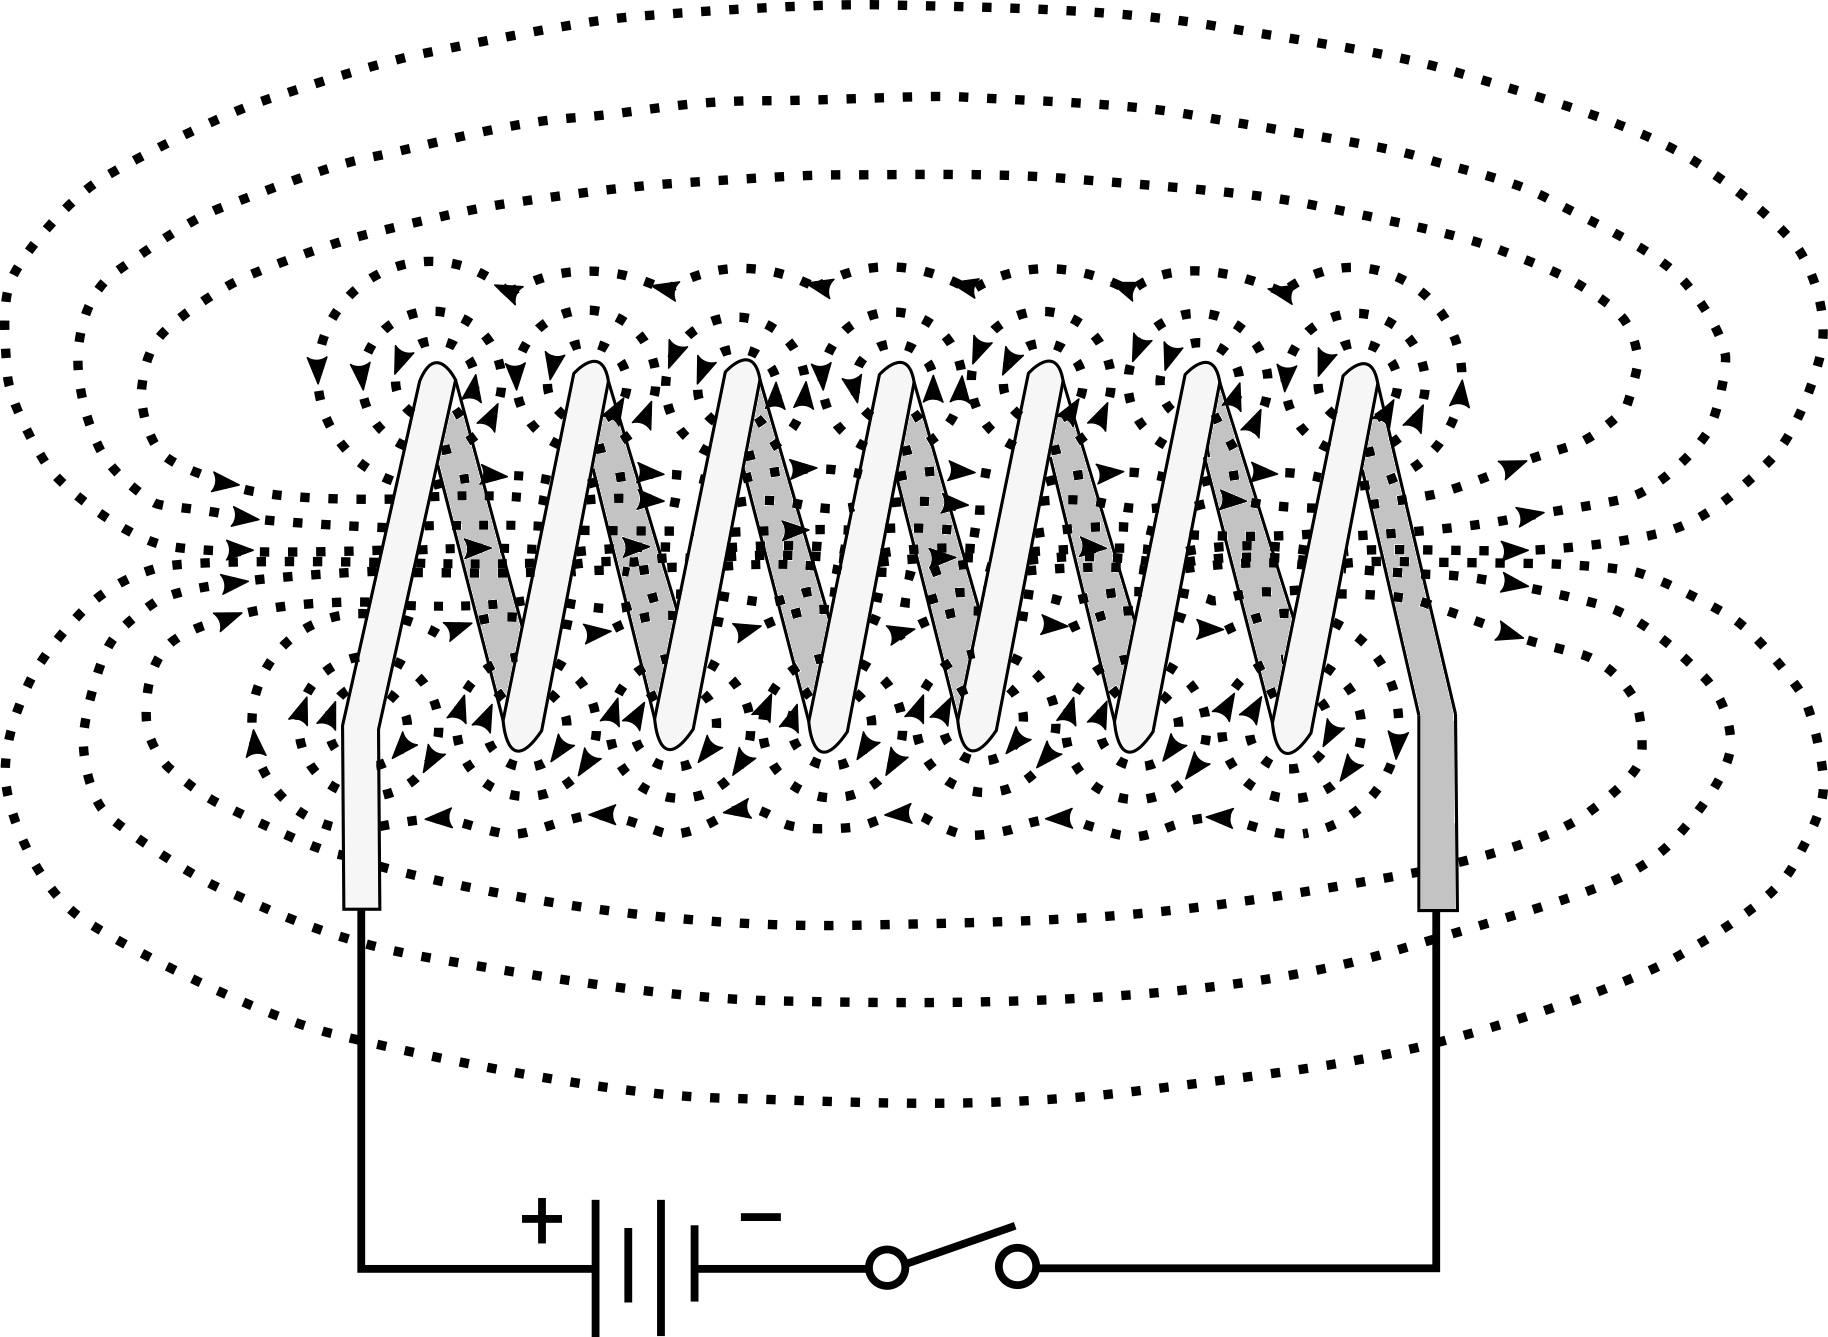
\includegraphics[scale=0.32]{grafiken/spule magnetfeld.PNG}}
\justify
Ein durch ein Leiter fließender Strom erzeugt ein kreisrundes Magnetfeld um den Leiter (die Richtung kann man mit der Rechten-Hand-Regel bestimmen; Daumen: Fließrichtung Elektronen, Finger: Kreisrichtung). Die Bauart einer einfachen Spule erlaubt ein annähernd homogenes Magnetfeld in Längsrichtung der Spule. Oft befindet sich im inneren ein Eisenkern um das Magnetfeld zusätzlich zu verstärken.\\
Die \textbf{Induktivität} ist die Fähigkeit einer Spule durch das Magnetfeld eine Spannung zu erzeugen.\\
Eine gängige Analogie zum verstehen, was in einer Spule im Stromkreis passiert ist die des \href{https://www.youtube.com/watch?v=KSylo01n5FY}{\textit{Wasserrads}}.
\[\text{Magnetischer Fluss } \Phi = \int B \, dA = L \cdot I \hspace{2cm} \text{Durchflutungsgesetz }I = \oint_s H \, ds\]
\[\text{Magnetische Energie } W = \frac{1}{2}LI^2\]
\end{mdframed}
\vspace{0.8\baselineskip}

\begin{mdframed}
\centering
\vspace{0.2\baselineskip}
\centering{\fbox{\textbf{Reihen- und Parallelschaltung}}}\\
\vspace{0.5\baselineskip}
\begin{tabular}{cc}
    &\\
    \makecell{\raisebox{-0.15\height}{\ctikzset{bipoles/thickness=1}
\begin{circuitikz}[line width=1pt, scale=0.7, transform shape, voltage shift = 0.5]
\large
\draw (0,0) to[L,l=$L_1$] (2,0) to[L,l=$L_2$] (4,0) to[L,l=$L_3$] (6,0);
\end{circuitikz}} \hspace{0.7\baselineskip} $L = L_1 + L_2 + L_3$} & \makecell{\raisebox{-0.4\height}{\ctikzset{bipoles/thickness=1}
\begin{circuitikz}[line width=1pt, scale=0.7, transform shape, voltage shift = 0.5]
\large
\draw (0,2) to[short,-*] (1,2) to[short,-*] (2,2) -- (3,2) to[L,name=L3] (3,0) to[short,-*] (2,0) to[short,-*] (1,0) -- (0,0);
\draw (1,2) to[L,name=L1] (1,0);
\draw (2,2) to[L,name=L2] (2,0);
\node[above, yshift=12pt, xshift=5pt] at (L1.n) {$L_1$};
\node[above, yshift=12pt, xshift=5pt] at (L2.n) {$L_2$};
\node[above, yshift=12pt, xshift=5pt] at (L3.n) {$L_3$};
\end{circuitikz}} \hspace{0.7\baselineskip} \scalebox{1.3}{$\frac{1}{L} = \frac{1}{L_1} + \frac{1}{L_3} + \frac{1}{L_3}$}} \\
    &\\
    Reihenschaltung & Parallelschaltung \\
\end{tabular}
\end{mdframed}
\vspace{0.7\baselineskip}

\begin{mdframed}
\centering
\vspace{0.2\baselineskip}
\fbox{\textbf{Ladevorgänge}}\\
\vspace{0.5\baselineskip}
\raisebox{-0.5\height}{\ctikzset{bipoles/thickness=1}
\begin{circuitikz}[line width=1pt, scale=0.9, transform shape, voltage shift = 0.5]
\large
\draw (0,0) to[vsource, v<=$U_0$, i=$I_0$] (0,3) to[short,-o] (0.5,3);
\draw [very thick](0.53,3) -- +(30:0.66);
\node [] at (0.9,3.7) {\text{\small\textbf{Laden}}};
\draw (1.2,3) to[short,o-] (1.2,3) to[R,l=$R_1$] (3.5,3);
\draw (3.5,3) to[short,*-o] (4.3,3);
\draw [very thick](4.33,3) -- +(30:0.66);
\draw (5,3) to[short,o-] (6,3);
\node [] at (4.9,3.7) {\text{\small\textbf{Entladen}}};
\draw (3.5,3) -- (3.5,2) to[L,l=$L$,v=$U_L$] (3.5,1) -- (3.5,0);
\draw (6,3) to[R,l=$R_2$] (6,0);
\draw (0,0) to[short,-*] (3.5,0) -- (6,0);
\end{circuitikz}}\\
\vspace{1\baselineskip}
\begin{mdframed}[linewidth=0.4mm]
\flushleft\textbf{\large Kennlinie}\\
\centering
\raisebox{-0.5\height}{\ctikzset{bipoles/thickness=1}
\begin{circuitikz}[line width=1pt, scale=1, transform shape, voltage shift = 0.5]
\large
\draw [->, very thick] (0,-1.7) -- (0,2) node[above]{$U_L$};
\draw [->, very thick] (0,0) -- (8,0) node[right]{$t$};
\node [] at (-0.5,1.7) {\small $U_0$};
\draw [densely dashed] (5,1.7) -- (5,-4.7);
\draw [densely dashed] (2.5,1.7) -- (2.5,-4.7);
\draw (-0.1,1.7) -- (0.1,1.7);
\draw [blue] (0,1.7) .. controls (0.5,0.7) and (0.9,0.05) .. (2.5,0);
\draw [blue] (2.5,0) -- (5,0);
\draw [blue] (5,-1.7) .. controls (5.4,-0.7) and (5.7,-0.05) .. (7.5,0);
\node [] at (1.3,-1.7) {\text{Laden}};
\node [] at (6.3,-1.7) {\text{Entladen}};
\draw [->, very thick] (0,-4.7) -- (0,-2.7) node[above]{$I$};
\draw [->, very thick] (0,-4.7) -- (8,-4.7) node[right]{$t$};
\draw [green!60!black] (0,-4.7) .. controls (0.5,-3.7) and (0.9,-3.05) .. (2.5,-3);
\draw [green!60!black] (5,-3) .. controls (5.4,-4) and (5.7,-4.65) .. (7.5,-4.7);
\draw [green!60!black] (2.5,-3) -- (5,-3);

\node [blue] at (1.6,-5.4) {$U_L(t) = U_0 \cdot e^{-\frac{R_1}{L}\cdot t}$};
\node [green!40!black] at (1.9,-6.4) {$I(t) = I_0 \cdot (1-e^{-\frac{R_1}{L} \cdot t})$};
\node [blue] at (6.8,-5.4) {$U_L(t) = -U_0 \cdot e^{-\frac{R_2}{L}\cdot t}$};
\node [green!40!black] at (6.4,-6.4) {$I(t) = I_0 \cdot e^{-\frac{R_2}{L}\cdot t}$};
\end{circuitikz}}
\begin{minipage}{0.4\textwidth}
Wenn der `Laden'-Schalter geschlossen wird entsteht abrupt eine selbstinduzierte Spannung an der Spule, was zu einem Anstieg am Stromfluss führt. In der Spule entsteht nun ein Magnetfeld. Im stationären Zustand, also falls der Stromfluss gleich bleibt, fließt der Strom durch die Spule als wäre es ein simpler Draht. Beim `Entladen' wird die im Magnetfeld gespeicherte Energie in elektrische Energie zurückgewandelt und es fließt wieder kurzfristig Strom bis die Spannung, also das Magnetfeld, sich abgebaut hat.\\ Das Zeitverhalten von Spannung und Strom ergibt sich durch:\\ 
\begin{mdframed}[linewidth=0.7mm]
\vspace{-0.8\baselineskip}
\begin{align*}
u_L(t) &= L\frac{di(t)}{dt} \\
i_L(t) &= \frac{1}{L}\int u(t)\,dt
\end{align*}
\end{mdframed}
\end{minipage}
\end{mdframed}
\vspace{0.6\baselineskip}
\end{mdframed}
\vspace{0.7\baselineskip}

\begin{mdframed}
\centering
\vspace{0.2\baselineskip}
\fbox{\textbf{Transformator}}\\
\vspace{0.5\baselineskip}
\justify
Ein Transformator ist ein elektrisches Bauteil, welches eine Eingangswechselspannung in eine höhere oder eine niedrigere Ausgangswechselspannung umwandeln kann. Ein typischer Trafo besteht aus zwei oder mehreren isolierten Kupferdrähten, die auf einem gemeinsamen Magnetkern aufgewickelt werden.
\justify
\centering
\vspace{0.5\baselineskip}
\raisebox{-0.5\height}{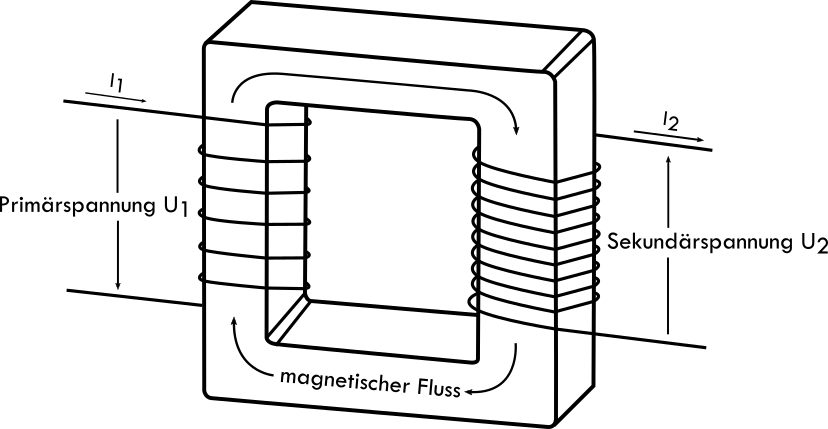
\includegraphics[scale=0.5]{grafiken/transformator schaubild.png}}
\hspace{1\baselineskip}
\begin{minipage}{0.3\linewidth}
\centering
\raisebox{-0.5\height}{\ctikzset{bipoles/thickness=1}
\begin{circuitikz}[line width=1pt, scale=1, transform shape, voltage shift = 0.5]
\Large
\draw (0,0) node[transformer core] {};
\end{circuitikz}}\\
\vspace{0.6\baselineskip}
\textit{Europäisches Schaltsymbol eines Transformators mit Eisenkern.}
\end{minipage}\\
\vspace{0.5\baselineskip}
\justify
Eine Wechselspannung auf der Primärseite des Transformators bewirkt einen wechselnden magnetischen Fluss im Kern. Dieser wechselnder Fluss induziert auf der Sekundärseite des Transformators eine Wechselspannung. Ob eine höhere oder niedrigere Spannung auf der Sekundärseite erzeugt wird, kann durch das Verhältnis der Windungen der Primärseite zur Sekundärseite festgelegt werden. Eine Faustregel: An der Seite mit mehr Windungen liegt eine größere Spannung an.
\justify
\centering
\begin{tabular}{cc}
     \begin{minipage}{0.25\textwidth}\vspace{0.35cm} Spannungsübersetzung \vspace{0.35cm}\end{minipage} & $\displaystyle \frac{U_2}{U_1} = \frac{n_2}{n_1}$ \\ 
     \begin{minipage}{0.25\textwidth}\vspace{0.35cm} Stromübersetzung \vspace{0.35cm}\end{minipage} & $\displaystyle \frac{I_2}{I_1} = \frac{U_1}{U_2} = \frac{n_1}{n_2}$ \\ 
     \begin{minipage}{0.25\textwidth}\vspace{0.35cm} Widerstandsübersetzung \vspace{0.35cm}\end{minipage} & $\displaystyle \frac{R_1}{R_2} = (\frac{n_1}{n_2})^2$ 
\end{tabular}
\end{mdframed}

\flushleft
\section{Wechselstrom / Wechselspannung}
\vspace{-0.8\baselineskip}
\begin{mdframed}
\centering
\vspace{0.2\baselineskip}
\centering{\fbox{\textbf{Einführung}}}\\
\vspace{0.5\baselineskip}
\justify
Da die Wechselstromlehre in dem Kurs gefühlt etwas schwamming besprochen wurde, will ich dieses Thema etwas ausführlicher angehen. Das heißt, dass ich versuchen werde zu zeigen, auf was für Probleme man schnell stößt, versucht man mit den herkömmlichen Methoden zu arbeiten. Des weiteren will ich die Idee der komplexen Impedanzen ein wenig herleiten, sodass da ein bisschen Verständnis aufgebaut werden kann.
\justify
\centering
\rule{0.6\textwidth}{0.5pt}\\
\justify
\indent Wir wollen nun von Gleichstrom zu Wechselstrom umschalten. Betrachtet werden jetzt die sinusförmigen, reinen Wechselgrößen. Das heißt, dass sich alle Spannungen und Ströme durch folgende Gleichungen beschreiben lassen:
\[u(t) = \hat{U} \cdot sin(\omega t + \varphi_U)\]
\[i(t) = \hat{I} \cdot sin(\omega t + \varphi_I)\]
mit:
\begin{align*}
    u(t),i(t) &= \text{zeitabhängige Spannung bzw. Strom}\\
    \hat{U},\hat{I} &= \text{Amplitude von Spannung bzw. Strom}\\
    \omega &= \text{Kreisfrequenz}\\
    \varphi_U,\varphi_I &= \text{Phase von Spannung bzw. Strom zum Zeitpunkt t = 0}
\end{align*}
\flushleft Die Größen können in folgender Abbildung dargestellt werden:\\
\vspace{1\baselineskip}
\centering
\raisebox{-0.5\height}{\ctikzset{bipoles/thickness=1}
\begin{circuitikz}[line width=1pt, scale=1, transform shape, voltage shift = 0.5]
\large
\draw [->, very thick] (0,-1.5) -- (0,1.5) node[above]{$U$};
\draw [->, very thick] (-1,0) -- (8,0) node[right]{$t$};
\draw[ultra thick] (-0.5,0) sin (0.5,1);
\draw[ultra thick] (0.5,1) cos (1.5,0);
\draw[ultra thick] (1.5,0) sin (2.5,-1);
\draw[ultra thick] (2.5,-1) cos (3.5,0);
\draw[ultra thick] (3.5,0)  sin (4.5,1);
\draw[ultra thick] (4.5,1) cos (5.5,0);
\draw[ultra thick] (5.5,0) sin (6.5,-1);
\draw[ultra thick] (6.5,-1) cos (7.5,0);
\draw[densely dashed] (-1,1) -- (1.5,1);
\draw[Latex-Latex] (-0.9,0) -- (-0.9,1);
\node[] at (-1.2,0.5) {$\hat{U}$};
\draw[Latex-Latex] (0.5,1.2) -- (4.5,1.2);
\node[] at (2.5,0.9) {$T$};
\draw[densely dashed] (0.5,0.5) -- (0.5,1.5);
\draw[densely dashed] (4.5,0.5) -- (4.5,1.5);
\draw[densely dashed] (-0.5,0.5) -- (-0.5,-0.5);
\draw[latex-latex] (-0.5,-0.2) -- (0,-0.2);
\node[] at (-0.25,-0.5) {$\varphi_U$};
\node[] at (3.5,-1.5) {\text{\footnotesize Zeitliche Darstellung einer Wechselspannung}};
\end{circuitikz}}
\vspace{1\baselineskip}
\justify
Die Spannungsamplitude $\hat{U}$ und die Phase $\varphi_U$ können wir unmittelbar aus dem Bild ablesen. Für die Kreisfrequenz gilt:
\begin{align*}
    T &= \text{ Periodendauer}\\
    f &= \frac{1}{T} \text{ Frequenz}\\
    \omega &= 2\pi f \text{ Kreisfrequenz}
\end{align*}
\flushleft Eine Darstellung im Zeigerdiagramm ist anschaulich und sinnvoll:\\
\centering
\vspace{1\baselineskip}
\raisebox{-0.5\height}{\ctikzset{bipoles/thickness=1}
\begin{circuitikz}[line width=1pt, scale=1, transform shape, voltage shift = 0.5]
\large
\draw [->, very thick] (0,-2) -- (0,2) node[above]{$U,I$};
\draw [->, very thick] (-1,0) -- (8,0) node[right]{$t$};
%Voltage sine
\draw[ultra thick, blue] (-0.5,0) sin (0.5,1);
\draw[ultra thick, blue] (0.5,1) cos (1.5,0);
\draw[ultra thick, blue] (1.5,0) sin (2.5,-1);
\draw[ultra thick, blue] (2.5,-1) cos (3.5,0);
\draw[ultra thick, blue] (3.5,0)  sin (4.5,1);
\draw[ultra thick, blue] (4.5,1) cos (5.5,0);
\draw[ultra thick, blue] (5.5,0) sin (6.5,-1);
\draw[ultra thick, blue] (6.5,-1) cos (7.5,0);
%Current sine
\draw[ultra thick, red] (-0.5,-1.7) cos (0.5,0);
\draw[ultra thick, red] (0.5,0) sin (1.5,1.7);
\draw[ultra thick, red] (1.5,1.7) cos (2.5,0);
\draw[ultra thick, red] (2.5,0) sin (3.5,-1.7);
\draw[ultra thick, red] (3.5,-1.7) cos (4.5,0);
\draw[ultra thick, red] (4.5,0)  sin (5.5,1.7);
\draw[ultra thick, red] (5.5,1.7) cos (6.5,0);
\draw[ultra thick, red] (6.5,0) sin (7.5,-1.7);
%Zeigerdiagramm
\draw[->, very thick] (-5,0) -- (-1,0);
\node[] at (-1,0.3) {$x$};
\draw[->, very thick] (-3,-2) -- (-3,2) node[above]{$y$};
\draw[very thick, red] (-3,0) circle (1.7);
\draw[very thick, blue] (-3,0) circle (1);
\draw[densely dashed, red] (0,-1.2) -- (-1.8,-1.2);
\draw[-latex, very thick, red] (-3,0) -- (-1.8,-1.2);
\node[red] at (-2.3,-1.1) {$\hat{I}$};
\draw[densely dashed, red] (-3,-1.7) -- (7.5,-1.7);
\draw[densely dashed, red] (-3,1.7) -- (7.5,1.7);
\draw[densely dashed, blue] (0,0.75) -- (-2.3,0.75);
\draw[-latex, very thick, blue] (-3,0) -- (-2.3,0.75);
\node[blue] at (-2.7, 0.65) {$\hat{U}$};
\draw[densely dashed, blue] (-3,1) -- (7.5,1);
\draw[densely dashed, blue] (-3,-1) -- (7.5,-1);
\node[] at (2,-2.5) {\text{\footnotesize Gemeinsame Darstellung von Strom und Spannung im Zeigerdiagramm}};
\end{circuitikz}}\\
\vspace{1\baselineskip}
\justify
In der Regel werden zeitabhängige Größen mit Kleinbuchstaben bezeichnet und zeitunhabhängige Größen mit Großbuchstaben. Die Länge des Zeigers entspricht der Amplitude und wird bei der Spannung in Volt gemessen und beim Strom in Ampere. Zum Zeitpunkt t = 0 hat der Zeiger den Winkel $\varphi_U$ und $\varphi_I$ mit der x-Achse (in der Regel in Bogenmaß). Der Zeiger dreht sich mit der Kreisfrequenz $\omega$ herum. Die Momentanwerte der Spannung $u(t)$ und des Stroms $i(t)$ erhält man jederzeit durch Projektion auf die y-Achse. \\
\justify
\vspace{2\baselineskip}
\centering{\fbox{\textbf{Modellieren komplexer Schaltungen}}}\\
\vspace{0.7\baselineskip}
\justify
Jetzt will ich zeigen, wieso die komplexen Zahlen in der Elektrotechnik so wichtig sind. Mit den bereits kennengelernten Tools, lassen sich zwar komplexere Schaltungen beschreiben und modellieren, nur wird es dann mathematisch sehr schnell hässlich und schwierig. Betrachten wir eine Schaltung, welche einen Widerstand, eine Spule und einen Kondensator beinhaltet:\\
\justify
\centering
\raisebox{-0.5\height}{\ctikzset{bipoles/thickness=1}
\begin{circuitikz}[line width=1pt, scale=0.9, transform shape, voltage shift = 0.5]
\large
\draw (0,0) to[vsource, v<=$U_0$] (0,3) to[short,-o] (0.5,3);
\draw [very thick](0.53,3) -- +(30:0.66);
\draw (1.2,3) to[short,o-] (1.2,3) to[R,l=$\color{red!50!black}R$] (4,3);
\draw (4,3) -- (4,2) to[L,l=$\color{green!50!black}L$] (4,1) -- (4,0);
\draw (4,0) to[C,l=$\color{blue!50!black}C$] (0,0);
\draw [thick] (3,1.6) arc (0:160:1);
\draw [thick, ->] (3,1.6) arc (360:200:1);
\end{circuitikz}}
\hspace{2\baselineskip}
\begin{minipage}{0.6\textwidth}
\justify
Hier haben wir eine RLC-Schaltung mit einer Gleichspannungsquelle. Mit der kirchhoffschen Maschengleichung können wir schreiben:
\[U_0 - \textcolor{red!50!black}{R \cdot i} - \textcolor{green!50!black}{L\frac{di(t)}{dt}} - \textcolor{blue!50!black}{\frac{1}{C}\int i(t)\,dt} = 0\]
Diese Gleichung bringt uns in der Form noch nicht viel. Sie muss vereinfacht werden, indem das Integral aufgelöst werden muss. Dafür differenzieren wir die Gleichung nach t und schreiben um:
\[L\frac{d^2i(t)}{dt^2}+R\frac{di(t)}{dt}+\frac{1}{C}i(t) = 0\]
Das ist eine homogene Differentialgleichung zweiter Ordnung und kann mit den Tools aus Mathe 3 gelöst werden.
\vspace{1\baselineskip}
\end{minipage}
\begin{minipage}{0.55\textwidth}
Jetzt nehmen wir die gleiche Schaltung, entfernen den Schalter und ersetzen die Gleichspannungsquelle mit einer Wechselspannung. Die Quelle kann mathematisch als $U_0 \,cos(\omega t)$ beschrieben werden. Nach Kirchhoff gilt:
\[U_0\,cos(\omega t) - R \cdot i - L\frac{di(t)}{dt} - \frac{1}{C}\int i(t)\,dt = 0\]
Differenzieren nach t:
\[L\frac{d^2i(t)}{dt^2}+R\frac{di(t)}{dt}+\frac{1}{C}i(t) = \omega U_0\,sin(\omega t)\]
Das ist eine inhomogene Differentialgleichung zweiter Ordnung und kann mit der Variation der Konstanten gelöst werden.
\vspace{1\baselineskip}
\end{minipage}
\hspace{1\baselineskip}
\raisebox{-0.5\height}{\ctikzset{bipoles/thickness=1}
\begin{circuitikz}[line width=1pt, scale=0.9, transform shape, voltage shift = 0.5]
\large
\draw (0,0) to[vsourcesin, v<=$U_0\,cos(\omega t)$] (0,3);
\draw (0,3) to[R,l=$R$] (4,3);
\draw (4,3) -- (4,2) to[L,l=$L$] (4,1) -- (4,0);
\draw (4,0) to[C,l=$C$] (0,0);
\draw [thick] (3,1.6) arc (0:160:1);
\draw [thick, ->] (3,1.6) arc (360:200:1);
\end{circuitikz}}
\justify
Wie man sieht, ist dieser Ansatz mathematisch gesehen nicht sehr vielversprechend. Es wird schlimmer mit der Anzahl an Komponenten und der Größe der Schaltung. Auch bei Spannungsquellen, die nicht sinusartig sind wie beispielsweise eine Rechteck- oder eine Sägezahnschwingung. Diese müssten über eine Fourierreihe ausgedrückt werden, was die Gleichungen umso unschöner machen. Mit diesem Ansatz stößt man schnell auf einige Schwierigkeiten bei der Modellierung. Man macht sich deshalb Gebrauch der \textbf{komplexen Zahlen} und dem Konzept der komplexen \textbf{Impedanzen}.
\end{mdframed}
\vspace{0.8\baselineskip}

\begin{mdframed}
\centering
\vspace{0.2\baselineskip}
\centering{\fbox{\textbf{Komplexe Zahlen}}}\\
\vspace{0.2\baselineskip}
\justify
Das Konzept der komplexen Zahlen ist aus Mathe 3 bekannt, deshalb belasse ich es hier bei einer knappen Formelsammlung. Die Elektrotechniker bezeichnen im Gegensatz zu den Mathematikern die komplexe Einheit als \textit{j}, da der Buchstabe i für den elektrischen Strom bereits vergeben ist.
\[j^2 = -1 \hspace{1\baselineskip},\hspace{1\baselineskip} j = \sqrt{-1}\]
\[\underline{z} = a + j \cdot b = r(cos\varphi + j \cdot sin\varphi) = re^{j\varphi} \hspace{1\baselineskip},\hspace{1\baselineskip} \underline{z}^* = a - j \cdot b\]
\centering
\raisebox{-0.5\height}{\ctikzset{bipoles/thickness=1}
\begin{circuitikz}[line width=1pt, scale=1, transform shape, voltage shift = 0.5]
\draw[-Latex, very thick] (0,-0.3) -- (0,1.5) node[above]{\small $Im(\underline{z})$};
\draw[-Latex, very thick] (-0.3,0) -- (1.5,0) node[right]{\small $Re(\underline{z})$};
\draw (0,0) -- (1,1);
\draw[densely dashed] (0,1) -- (1,1);
\draw[densely dashed] (1,0) -- (1,1);
\node[] at (1,-0.2) {a};
\node[] at (-0.2,1) {b};
\node[] at (1.1,1.1) {z};
\node[] at (0.4,0.7) {|z|};
\draw[-latex] (0.5,0) arc (0:45:0.5);
\node[] at (0.3,0.1) {\scriptsize $\varphi$};
\end{circuitikz}}
$\begin{aligned}[t]
    Betrag&: r = |z| = \sqrt{a^2+b^2}\\
    Phase&: \varphi = arctan(\frac{b}{a})
\end{aligned}$
\end{mdframed}
\vspace{0.8\baselineskip}

\begin{mdframed}
\centering
\vspace{0.2\baselineskip}
\centering{\fbox{\textbf{Wechselspannung mit komplexen Zahlen}}}\\
\vspace{0.2\baselineskip}
\justify
In der Elektrotechnik wird ein Konzept bei der Wechselstromlehre verwendet, welches erlaubt Kondensatoren und Spulen als `spezielle Arten' von Widerständen zu definieren. Dadurch kann man bei der Analyse alle Gleichstromgesetze von vorher auch für Wechselstromnetze verwenden, und das ganz ohne zeitabhängige Differentialgleichungen.\\ \\ 
In einer Schaltung, mit einer sinusartigen Wechselstrom- oder Wechselspannungsquelle, sind alle Ströme und Spannungen innerhalb dieser Schaltung ebenfalls sinusartig.
Es ist bekannt, dass komplexe Zahlen sinusartiges Verhalten im komplexen Raum aufweisen. Wir machen uns zu Nutze, dass mit komplexen Zahlen das Lösen trigonometrischer Aufgaben wesentlich einfacher ist. Es kann schnell verwirren, wieso ein `imaginärer' Teil von Nöten ist, es gibt schließlich tatsächlich keinen imaginären Strom oder keine imaginäre Spannung. Grund ist, dass durch diese Beschreibung der Mechanismus eingeführt wird, welcher die Phase berücksichtigt. \\ \\
Nun kommt der entscheidende Schritt, bei dem die Spannungen und Ströme durch komplexe Zahlen beschrieben werden. Zu Beginn hieß es:
\[u(t) = \hat{U} \cdot sin(\omega t + \varphi)\]
Nun definieren wir:
\[\underline{u}(t) = \hat{U} \cdot cos(\omega t + \varphi) + j \cdot \hat{U} \cdot sin(\omega t + \varphi)\]
Offenbar gilt:
\[u(t) = Im(\underline{u}(t))\]
Das entspricht genau der Beobachtung von oben, dass der Momentanwert der Spannung durch die Projektion auf die y-Achse (also dem Imaginärteil) beobachtbar ist. Weiter gilt:
\justify
\centering
\hspace{5\baselineskip}
\begin{minipage}{0.4\textwidth}
\begin{align*}
    \underline{u}(t) &= \hat{U} \cdot cos(\omega t + \varphi) + j \cdot \hat{U} \cdot sin(\omega t + \varphi)\\
    &= \hat{U} \cdot e^{j(\omega t + \varphi)}\\
    &= \textcolor{blue}{\hat{U} \cdot e^{j\varphi}} \cdot e^{j\omega t}\\
    &= \textcolor{blue}{\underline{\hat{U}}} \cdot e^{j\omega t}
\end{align*}
\end{minipage}
\hspace{2\baselineskip}
\begin{minipage}{0.3\textwidth}
\raisebox{-0.5\height}{\ctikzset{bipoles/thickness=1}
\begin{circuitikz}[line width=1pt, scale=1.1, transform shape, voltage shift = 0.5]
\draw[-Latex, very thick] (0,-1.6) -- (0,1.7) node[above]{\small $Im(\underline{z})$};
\draw[-Latex, very thick] (-1.6,0) -- (1.7,0) node[right]{\small $Re(\underline{z})$};
\draw[-latex, ultra thick] (0,0) -- (1,1);
\draw[densely dashed] (0,1) -- (1,1);
\draw[densely dashed] (1,0) -- (1,1);
\draw[dashed] (0,0) circle (1.414);
\node[] at (1.2,1.2) {$\underline{\hat{U}}$};
\draw[-latex] (0.7,0) arc (0:45:0.7);
\node[] at (0.4,0.17) {\small $\varphi$};
\draw[-latex] (0.6,0.6) arc (45:220:0.849);
\node[] at (-0.6,-0.7) {\small $\omega t$};
\end{circuitikz}}
\end{minipage}\\
\vspace{0.5\baselineskip}
\justify
Die zeitunabhängigen Größen wurden im Faktor $\underline{\hat{U}}$ zusammengefasst, den wir \textit{komplexe Amplitude} nennen. Der Zeiger dieser komlexen Amplitute ist im Zeigerdiagramm wieder zu finden mit der Länge $\hat{U}$ und dem Winkel $\varphi$. Dieser Zeiger rotiert nun gegen den Uhrzeigersinn mit der Winkelfrequenz $\omega$.\\
\centering
\rule{0.5\textwidth}{0.5pt}\\
\justify
Jetzt, da wir den komplexen Ausdruck für die Spannung haben, können wir einen Widerstand, einen Kondensator oder eine Spule anschließen, und eine komplexe Gleichung für den Strom finden, der durch die Komponenten fließt. Es werden beide Größen Strom und Spannung im Zeigerdiagramm geplottet.\\ \\
\vspace{0.5\baselineskip}
\begin{tabular}{p{0.15\textwidth}p{0.75\textwidth}}
     \textit{Widerstand}: & Strom und Spannung sind in Phase ($\varphi = 0^{\circ}$). Im Schaubild liegen daher die beiden Zeiger der Spannung und des Stroms aufeinander. \\
     \textit{Kondensator}: & Der Strom eilt der Spannung um $\varphi = 90^{\circ}$ vor. Der Winkel wird in der Regel vom Spannungszeiger aus festgelegt. Merksatz: \textit{Im \textbf{Kondensator} eilt der \textbf{Strom vor}}.\\
     \textit{Spule}: & Der Strom ist außer Phase mit der Spannung um $\varphi = -90^{\circ}$, d.h. der Strom geht der Spannung hinterher. Merksatz: \textit{In \textbf{Induktivitäten} tut sich der \textbf{Strom verspäten}}.
\end{tabular}\\
\centering
\vspace{1\baselineskip}
\raisebox{-0.5\height}{\ctikzset{bipoles/thickness=1}
\begin{circuitikz}[line width=1pt, scale=0.87, transform shape, voltage shift = 0.5]
\large
\definecolor{ceruleanblue}{rgb}{0.16, 0.32, 0.75}
\definecolor{asparagus}{rgb}{0.53, 0.66, 0.42}
%Schaltung
\node[] at (1.2,1.8) {\Large \text{\textbf{Widerstand}}};
\draw (0,-1) to[vsourcesin, v<=$\underline{\hat{U}} \cdot e^{j\omega t}$] (0,1) -- (2.5,1) to[R,l=$R$,i=$I$] (2.5,-1) -- (0,-1);
\node[] at (1.5,-1.7) {\Large $I_R = \frac{U}{R} = \frac{\underline{\hat{U}} e^{j\omega t}}{R}$};

%Zeigerdiagramm
\draw[->] (4,0) -- (8,0) node[right] {$x$};
\draw[->] (6,-2) -- (6,2) node[above]{$y$};
\draw[ceruleanblue] (6,0) circle (1.7);
\draw[asparagus] (6,0) circle (1);
\draw[-Latex,ultra thick,ceruleanblue] (6,0) -- (7.7,0);
\draw[-Latex,ultra thick,asparagus] (6,0) -- (7,0);
\draw[very thin] (6.5,-0.2) -- (7.5,-1.5);
\node[] at (7.6,-1.7) {\small\text{Strom}};
\draw[very thin] (7.2,0.2) -- (7.7,1.5);
\node[] at (7.8,1.7) {\small\text{Spannung}};
\draw[-latex] (5.6,1.9) arc (95:175:1.65);
\node[] at (4.5,1.8) {$\omega t$};

%Graph
\draw[->, very thick] (9,0) -- (17.5,0) node[right]{$t$};
\draw[->, very thick] (9,-2) -- (9,2) node[above]{$\textcolor{ceruleanblue}{U},\textcolor{asparagus}{I}$};
    %Spannung
\draw[very thick, ceruleanblue] (9,0) sin (10,1.7);
\draw[very thick, ceruleanblue] (10,1.7) cos (11,0);
\draw[very thick, ceruleanblue] (11,0) sin (12,-1.7);
\draw[very thick, ceruleanblue] (12,-1.7) cos (13,0);
\draw[very thick, ceruleanblue] (13,0)  sin (14,1.7);
\draw[very thick, ceruleanblue] (14,1.7) cos (15,0);
\draw[very thick, ceruleanblue] (15,0) sin (16,-1.7);
\draw[very thick, ceruleanblue] (16,-1.7) cos (17,0);
    %Strom
\draw[very thick, asparagus] (9,0) sin (10,1);
\draw[very thick, asparagus] (10,1) cos (11,0);
\draw[very thick, asparagus] (11,0) sin (12,-1);
\draw[very thick, asparagus] (12,-1) cos (13,0);
\draw[very thick, asparagus] (13,0)  sin (14,1);
\draw[very thick, asparagus] (14,1) cos (15,0);
\draw[very thick, asparagus] (15,0) sin (16,-1);
\draw[very thick, asparagus] (16,-1) cos (17,0);

\end{circuitikz}}\\
\raisebox{-0.5\height}{\ctikzset{bipoles/thickness=1}
\begin{circuitikz}[line width=1pt, scale=0.87, transform shape, voltage shift = 0.5]
\large
\definecolor{ceruleanblue}{rgb}{0.16, 0.32, 0.75}
\definecolor{asparagus}{rgb}{0.53, 0.66, 0.42}
%Schaltung
\node[] at (1.2,1.8) {\Large \text{\textbf{Kondensator}}};
\draw (0,-1) to[vsourcesin, v<=$\underline{\hat{U}} \cdot e^{j\omega t}$] (0,1) -- (2.5,1) to[C,l=$C$,i=$I$] (2.5,-1) -- (0,-1);
\node[] at (1.5,-1.7) {\Large $I_C = C\frac{dU}{dt} = j\omega C \cdot \underline{\hat{U}}e^{j\omega t}$};

%Zeigerdiagramm
\draw[->] (4,0) -- (8,0) node[right] {$x$};
\draw[->] (6,-2) -- (6,2) node[above]{$y$};
\draw[ceruleanblue] (6,0) circle (1.7);
\draw[asparagus] (6,0) circle (1);
\draw[-Latex,ultra thick,ceruleanblue] (6,0) -- (7.7,0);
\draw[-Latex,ultra thick,asparagus] (6,0) -- (6,1);
\draw[-latex] (6.7,0) arc (0:80:0.7);
\node[] at (6.35,0.2) {\small $90^{\circ}$};

%Graph
\draw[->, very thick] (9,0) -- (17.5,0) node[right]{$t$};
\draw[->, very thick] (9,-2) -- (9,2) node[above]{$\textcolor{ceruleanblue}{U},\textcolor{asparagus}{I}$};
    %Spannung
\draw[very thick, ceruleanblue] (9,0) sin (10,1.7);
\draw[very thick, ceruleanblue] (10,1.7) cos (11,0);
\draw[very thick, ceruleanblue] (11,0) sin (12,-1.7);
\draw[very thick, ceruleanblue] (12,-1.7) cos (13,0);
\draw[very thick, ceruleanblue] (13,0)  sin (14,1.7);
\draw[very thick, ceruleanblue] (14,1.7) cos (15,0);
\draw[very thick, ceruleanblue] (15,0) sin (16,-1.7);
\draw[very thick, ceruleanblue] (16,-1.7) cos (17,0);
    %Strom
\draw[very thick, asparagus] (9,1) cos (10,0);
\draw[very thick, asparagus] (10,0) sin (11,-1);
\draw[very thick, asparagus] (11,-1) cos (12,0);
\draw[very thick, asparagus] (12,0)  sin (13,1);
\draw[very thick, asparagus] (13,1) cos (14,0);
\draw[very thick, asparagus] (14,0) sin (15,-1);
\draw[very thick, asparagus] (15,-1) cos (16,0);
\draw[very thick, asparagus] (16,0) sin (17,1);

\draw[densely dashed, thin] (13,2.1) -- (13,0.5);
\draw[densely dashed, thin] (14,2.1) -- (14,0.5);
\draw[latex-latex] (13,2) -- (14,2); 
\node[] at (13.6,2.3) {\small $90^{\circ}$};

\end{circuitikz}}\\
\raisebox{-0.5\height}{\ctikzset{bipoles/thickness=1}
\begin{circuitikz}[line width=1pt, scale=0.87, transform shape, voltage shift = 0.5]
\large
\definecolor{ceruleanblue}{rgb}{0.16, 0.32, 0.75}
\definecolor{asparagus}{rgb}{0.53, 0.66, 0.42}
%Schaltung
\node[] at (1.2,1.8) {\Large \text{\textbf{Spule}}};
\draw (0,-1) to[vsourcesin, v<=$\underline{\hat{U}} \cdot e^{j\omega t}$] (0,1) -- (2.5,1) to[L,l=$L$,i=$I$] (2.5,-1) -- (0,-1);
\node[] at (1.5,-1.7) {\Large $I_L = \frac{1}{L} \int U \, dt = -j\frac{1}{\omega L} \cdot \underline{\hat{U}}e^{j\omega t}$};

%Zeigerdiagramm
\draw[->] (4,0) -- (8,0) node[right] {$x$};
\draw[->] (6,-2) -- (6,2) node[above]{$y$};
\draw[ceruleanblue] (6,0) circle (1.7);
\draw[asparagus] (6,0) circle (1);
\draw[-Latex,ultra thick,ceruleanblue] (6,0) -- (7.7,0);
\draw[-Latex,ultra thick,asparagus] (6,0) -- (6,-1);
\draw[latex-] (6,-0.7) arc (270:360:0.7);
\node[] at (6.3,-0.2) {\small $-90^{\circ}$};

%Graph
\draw[->, very thick] (9,0) -- (17.5,0) node[right]{$t$};
\draw[->, very thick] (9,-2) -- (9,2) node[above]{$\textcolor{ceruleanblue}{U},\textcolor{asparagus}{I}$};
    %Spannung
\draw[very thick, ceruleanblue] (9,0) sin (10,1.7);
\draw[very thick, ceruleanblue] (10,1.7) cos (11,0);
\draw[very thick, ceruleanblue] (11,0) sin (12,-1.7);
\draw[very thick, ceruleanblue] (12,-1.7) cos (13,0);
\draw[very thick, ceruleanblue] (13,0)  sin (14,1.7);
\draw[very thick, ceruleanblue] (14,1.7) cos (15,0);
\draw[very thick, ceruleanblue] (15,0) sin (16,-1.7);
\draw[very thick, ceruleanblue] (16,-1.7) cos (17,0);
    %Strom
\draw[very thick, asparagus] (9,-1) cos (10,0);
\draw[very thick, asparagus] (10,0) sin (11,1);
\draw[very thick, asparagus] (11,1) cos (12,0);
\draw[very thick, asparagus] (12,0) sin (13,-1);
\draw[very thick, asparagus] (13,-1) cos (14,0);
\draw[very thick, asparagus] (14,0)  sin (15,1);
\draw[very thick, asparagus] (15,1) cos (16,0);
\draw[very thick, asparagus] (16,0) sin (17,-1);

\draw[densely dashed, thin] (14,2.1) -- (14,0.5);
\draw[densely dashed, thin] (15,2.1) -- (15,0.5);
\draw[latex-latex] (14,2) -- (15,2); 
\node[] at (14.6,2.3) {\small $90^{\circ}$};

\end{circuitikz}}\\
\justify
\vspace{0.2\baselineskip}
Jetzt kommt der entscheidende Trick, welcher die Wechselstromlehre so angenehm zu handhaben macht. Nehmen wir nun die Spannung an jeder Komponente und dividieren diese mit der Stromstärke, bekommen wir folgendes:
\justify
\centering
\begin{tabular}{|p{0.2\textwidth}>{\raggedright\arraybackslash}p{0.6\textwidth}|}
    \hline
    \raisebox{-3.2\height}{\ctikzset{bipoles/thickness=1}
\begin{circuitikz}[line width=1pt, scale=0.6, transform shape, voltage shift = 0.5]
\Large
\draw (0,0) to[R] (2.5,0);
\end{circuitikz}} & \Large \[\underline{Z}_R = \frac{U}{I_R} = \frac{\underline{\hat{U}} e^{j\omega t}}{\frac{\underline{\hat{U}}}{R} \, e^{j\omega t}} = R\]\\\hline
    \raisebox{-2.2\height}{\ctikzset{bipoles/thickness=1}
\begin{circuitikz}[line width=1pt, scale=0.7, transform shape, voltage shift = 0.5]
\large
\draw (0,0) to[C] (2,0);
\end{circuitikz}} & \Large \[\underline{Z}_C = \frac{U}{I_C} = \frac{\underline{\hat{U}} e^{j\omega t}}{j \omega C \cdot \underline{\hat{U}} e^{j\omega t}} = \frac{1}{j \omega C} = -j \frac{1}{\omega C}\]\\\hline
    \raisebox{-2.8\height}{\ctikzset{bipoles/thickness=1}
\begin{circuitikz}[line width=1pt, scale=0.7, transform shape, voltage shift = 0.5]
\large
\draw (0,0) to[L] (2.5,0);
\end{circuitikz}} & \Large \[\underline{Z}_L = \frac{U}{I_L} = \frac{\underline{\hat{U}} e^{j\omega t}}{\frac{\underline{\hat{U}}}{j \omega L} \cdot e^{j \omega t}} = j \omega L\]\\\hline
\end{tabular}\\
\justify
Wie man sieht, verschwindet der hässliche $\underline{\hat{U}} e^{j\omega t}$ Term und übrig bleiben die sogenannten komplexen \textbf{Impedanzen} der Komponenten. Das ist der Trick, der uns erlaubt die unangenehmen Differentialgleichungen zu umgehen. Jetzt können wir Kondensator sowie Spulen wie \textbf{frequenzabhängige Widerstände} innerhalb einer sinusartigen wechselspannungbetriebenen Schaltung behandeln. Solange alle Spannungen, Ströme sowie Widerstände in komplexer Form ausgedrückt werden, können wir die alten Gesetze wie dem Ohm'schen Gesetz oder der kirchhoffschen Gleichungen problemlos weiter verwenden. Die Impedanz ist also einfach nur eine allgemeine Art der Beschreibung von komplexen Widerständen und kann einfach nur resistiv, nur kapazitiv, nur induktiv oder eben eine Kombination von allen Dreien sein. Jetzt wollen wir die RLC-Schaltung von vorhin noch einmal mit den komplexen Impedanzen beschreiben:
\justify
\centering
\raisebox{-0.2\height}{\ctikzset{bipoles/thickness=1}
\begin{circuitikz}[line width=1pt, scale=0.7, transform shape, voltage shift = 0.5]
\large
\draw (0,0) to[R,l=$R$] (2,0) to[L,l=$L$] (4,0) to[C,l=$C$] (6,0);
\end{circuitikz}}
\hspace{1\baselineskip}
$\underline{Z} = R + \underline{Z}_C + \underline{Z}_L = R - j\frac{1}{\omega C} + j\omega L = R + j(\omega L - \frac{1}{\omega C})$\\
\justify
Es ist direkt zu erkennen, dass dieser Ansatz um einiges einfacher ist als eine Differentialgleichung. Jetzt lässt sich ganz einfach frequenzabhängig der Strom berechnen. \\
Auch die Regeln der Reihenschaltung oder Parallelschaltung (von Widerständen) ist übertragbar auf die Impedanzen, genauso der Spannungs- und Stromteiler.\\ \\ \\
Zum festigen einige Beispielschaltungen und deren komplexen Impedanzen:
\justify
\centering
\raisebox{-0.2\height}{\ctikzset{bipoles/thickness=1}
\begin{circuitikz}[line width=1pt, scale=0.7, transform shape, voltage shift = 0.5]
\large
\draw (0,0) to[R,l=$R$] (2,0) to[C,l=$C$] (4,0);
\node[] at (-0.5,0) {\Large \text{\textbf{a.}}};
\end{circuitikz}}
\raisebox{-0.2\height}{\ctikzset{bipoles/thickness=1}
\begin{circuitikz}[line width=1pt, scale=0.7, transform shape, voltage shift = 0.5]
\large
\draw (0,0) to[short,-*] (0.5,0) -- (0.5,0.5) to[L,l=$L$] (2.5,0.5) to[short,-*] (2.5,0) -- (3,0);
\draw (0.5,0) -- (0.5,-0.5) to[R,l=$R$] (2.5,-0.5) -- (2.5,0);
\node[] at (-0.5,0) {\Large \text{\textbf{b.}}};
\end{circuitikz}}
\raisebox{-0.2\height}{\ctikzset{bipoles/thickness=1}
\begin{circuitikz}[line width=1pt, scale=0.7, transform shape, voltage shift = 0.5]
\large
\draw (0,0) to[short,-*] (0.5,0) -- (0.5,0.5) to[C,l=$C$] (4.5,0.5) to[short,-*] (4.5,0) -- (5,0);
\draw (0.5,0) -- (0.5,-0.5) to[R,l=$R$] (2.5,-0.5) to[L,l=$L$] (4.5,-0.5) -- (4.5,0);
\node[] at (-0.5,0) {\Large \text{\textbf{c.}}};
\end{circuitikz}}
\raisebox{-0.2\height}{\ctikzset{bipoles/thickness=1}
\begin{circuitikz}[line width=1pt, scale=0.7, transform shape, voltage shift = 0.5]
\large
\draw (0,0) to[short,-*] (0.5,0) -- (0.5,0.5) to[R,l=$R_1$] (2.5,0.5) to[L,l=$L$] (4.5,0.5) to[short,-*] (4.5,0) -- (5,0);
\draw (0.5,0) -- (0.5,-0.5) to[R,l=$R_2$] (2.5,-0.5) to[C,name=C] (4.5,-0.5) -- (4.5,0);
\node[above,xshift=12pt,yshift=3pt] at (C) {$C$};
\node[] at (-0.5,0) {\Large \text{\textbf{d.}}};
\end{circuitikz}}\\
\vspace{1.5\baselineskip}
\rule{0.3\textwidth}{0.5pt}\\
\justify
\begin{minipage}{0.4\textwidth}
Lösungen:
\begin{enumerate}[label=(\alph*)]
\item $\displaystyle \underline{Z}_a = R-j\frac{1}{\omega C}$
\item $\displaystyle \underline{Z}_b = \frac{jR\omega L}{R + j\omega L}$
\item $\displaystyle \underline{Z}_c = \frac{\frac{L}{C}-j(\frac{R}{\omega C})}{R + j(\omega L - \frac{1}{\omega C})}$
\item $\displaystyle \underline{Z}_d = \frac{(R_1R_2 + \frac{L}{C}) + j(R_2 \omega L - \frac{R_1}{\omega C})}{(R_1 + R_2) + j(\omega L - \frac{1}{\omega C})}$
\end{enumerate}
\end{minipage}
\begin{minipage}{0.4\textwidth}
Jetzt lassen sich die Ausdrücke natürlich noch in Real- und Imaginärteil auflösen. Könnt ihr selber gerne probieren.
\end{minipage}\\
\par\vspace{0.5\baselineskip}
\centering
\end{mdframed}

\flushleft
\section{Sonstiges}
\vspace{-0.8\baselineskip}
\begin{mdframed}
\centering
\vspace{0.2\baselineskip}
\centering{\fbox{\textbf{Wie ist das mit der Stromrichtung?}}}\\
\vspace{0.2\baselineskip}
\justify
Vor langer Zeit (1750er) leistete Benjamin Franklin seine Pionierarbeit in der frühen Elektronik und führte erstmals die Konvention ein, den damals mysteriösen Dingen, die sich bewegten und Arbeit verrichteten, positive Ladungszeichen zuzuweisen. Nach Franklin bewegten sich im Leiter also positive Ladungsträger in der Richtung des heute universal verbreiteten konventionellen Stroms (von + nach -). 1897 entdeckte J.J. Thomson erstmals die unbekannten, negativ geladenen Partikel, die heute als Elektronen bekannt sind. Er steht mit seiner Aussage, dass negative Ladungsträger in entgegengesetzter Richtung fließen (von - nach +), der Franklins gegenüber. Mit der Zeit hat sich herausgestellt, dass Thomson recht hat und Franklin nicht. Die Konvention Franklins steht aber heute noch. Deshalb ist wichtig zu verstehen: \textbf{Wenn über die Stromstärke I und deren Richtung gesprochen wird, können wir einfach die Augen schließen und annehmen es bewegen sich positive Ladungen in der Leitung und den elektrischen Geräten und alles würde einwandfrei funktionieren. Negative Elektronen, die in eine Richtung gehen ist äquivalent zu positiver Ladung, die in die entgegengesetzte Richtung gehen. Man muss sich nur bewusst machen, dass die tatsächliche Bewegung negativer Elektronen, entgegengesetzt der Stromrichtung ist.}
\justify
\centering
\raisebox{-0.5\height}{\ctikzset{bipoles/thickness=1}
\begin{circuitikz}[line width=1pt, scale=1, transform shape, voltage shift = 0.5]
\Large
\draw (0,0) to[battery1,l=$_+ \, \, _-$] (3,0) -- (3,2) -- (0,2) -- (0,0);
\draw[green!60!black] (1,-0.5) -- (-0.5,-0.5) -- (-0.5,2.5);
\draw[green!60!black,-latex] (-0.5,2.5) -- (1,2.5);
\node[green!60!black] at (-2.3,1) {\text{\small konventioneller Strom}};
\draw[blue] (2,-0.5) -- (3.5,-0.5) -- (3.5,2.5);
\draw[blue,-latex] (3.5,2.5) -- (2,2.5);
\node[blue] at (4.5,1) {\text{\small Elektronen}};
\end{circuitikz}}
\raisebox{-0.5\height}{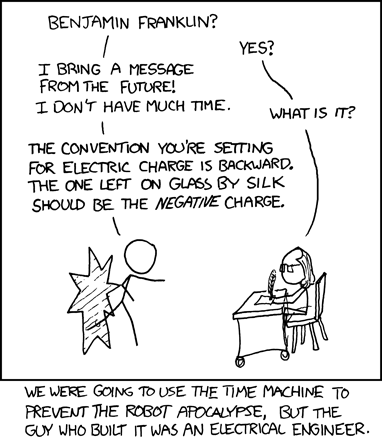
\includegraphics[scale=0.48]{grafiken/franklin comic.png}}
\hspace{2\baselineskip}
\end{mdframed}
\vspace{1.4\baselineskip}

\begin{mdframed}
\centering
\vspace{0.2\baselineskip}
\centering{\fbox{\textbf{Filter und Übertragungsfunktionen}}}\\
\vspace{0.2\baselineskip}
\justify
Durch spezielle Kombinationen von Widerständen, Kondensatoren und Spulen können Schaltungen entworfen werden, die in der Lage sind, bestimmte Frequenzen bzw. Signale durchzulassen, während andere abgewiesen werden. Im folgenden sind die einfachsten und wichtigsten Filter aufgelistet. Es wird auch mathematisch gezeigt, wieso es zu einem Durchlassen oder einer Sperre von bestimmten Frequenzen kommt. Wenn ein Filter gegeben ist und man nicht direkt erkennt, was für einer das sein soll, einfach die Übertragsfunktion $\frac{\underline{U}_A}{\underline{U}_E}$ aufstellen und die Funktion gegen 0 sowie $\infty$ laufen lassen. Dann sollte man sehr schnell erkennen, bei welchen Frequenzen der Filter sperrt und bei welchen er durchlässt.\\
\justify
\centering
\begin{tabular}{ccc}
     \raisebox{-0.5\height}{\ctikzset{bipoles/thickness=1}
\begin{circuitikz}[line width=1pt, scale=0.7, transform shape, voltage shift = 0.5]
\large
\draw (0,2) to[short,o-] (0.5,2) to[R,l=$R$] (3,2) to[short,-o] (5,2);
\draw (3,2) to[short,*-] (3,1.8) to[C,l=$C$] (3,0.2) to[short,-*] (3,0);
\draw (0,0) to[short,o-] (2.5,0) to[short,-o] (5,0);
\draw (0,2) to[open,v=$U_E$] (0,0);
\draw (5,2) to[open,v=$U_A$] (5,0);
\node[] at (2.5,-1) {\text{\textbf{RC - Tiefpass}}};
\end{circuitikz}} & \begin{minipage}{0.37\textwidth}$\displaystyle \underline{U}_E = (R + \frac{1}{j\omega C}) \cdot I \,\, , \,\, \underline{U}_A = \frac{1}{j\omega C} \cdot I \\ \frac{\underline{U}_A}{\underline{U}_E} = \frac{\frac{1}{j\omega C} \cdot I}{(R + \frac{1}{j\omega C}) \cdot I} = \frac{1}{1 + j\omega RC} \\ \lim_{\omega \to 0} \frac{1}{1 + j\omega RC} = 1 \,\, , \,\, \lim_{\omega \to \infty} \frac{1}{1 + j\omega RC} = 0$\end{minipage} & \multirow{2}{*}{\raisebox{-0.4\height}{\ctikzset{bipoles/thickness=1}
\begin{circuitikz}[line width=1pt, scale=0.9, transform shape, voltage shift = 0.5]
\large
\draw[-Latex, very thick] (0,0) -- (0,2) node[above]{$\frac{\underline{U}_A}{\underline{U}_E}$};
\draw[-Latex, very thick] (0,0) -- (4,0) node[right]{$\omega$};
\draw[rounded corners=4mm] (0,1.5) -- (1.8,1.5) -- (3.5,0);
\draw[densely dashed] (0,1.5) -- (3.8,1.5);
\draw (-0.15,1.5) -- (0.15,1.5);
\node[] at (-0.3,1.5) {$1$};
\end{circuitikz}}}\\
     
     \raisebox{-0.5\height}{\ctikzset{bipoles/thickness=1}
\begin{circuitikz}[line width=1pt, scale=0.7, transform shape, voltage shift = 0.5]
\large
\draw (0,2) to[short,o-] (0.5,2) to[L,l=$L$] (3,2) to[short,-o] (5,2);
\draw (3,2) to[short,*-] (3,1.8) to[R,l=$R$] (3,0.2) to[short,-*] (3,0);
\draw (0,0) to[short,o-] (2.5,0) to[short,-o] (5,0);
\draw (0,2) to[open,v=$U_E$] (0,0);
\draw (5,2) to[open,v=$U_A$] (5,0);
\node[] at (2.5,-1) {\text{\textbf{RL - Tiefpass}}};
\end{circuitikz}} & \begin{minipage}{0.37\textwidth}$\displaystyle \frac{\underline{U}_A}{\underline{U}_E} = \frac{R}{R + j\omega L} \\ \lim_{\omega \to 0} \frac{R}{R + j\omega L} = 1 \,\, , \,\, \lim_{\omega \to \infty} \frac{R}{R + j\omega L} = 0$\end{minipage} & \\ \hline
     
     \raisebox{-0.5\height}{\ctikzset{bipoles/thickness=1}
\begin{circuitikz}[line width=1pt, scale=0.7, transform shape, voltage shift = 0.5]
\large
\draw (0,2) to[short,o-] (0.5,2) to[C,l=$C$] (3,2) to[short,-o] (5,2);
\draw (3,2) to[short,*-] (3,1.8) to[R,l=$R$] (3,0.2) to[short,-*] (3,0);
\draw (0,0) to[short,o-] (2.5,0) to[short,-o] (5,0);
\draw (0,2) to[open,v=$U_E$] (0,0);
\draw (5,2) to[open,v=$U_A$] (5,0);
\node[] at (2.5,-1) {\text{\textbf{RC - Hochpass}}};
\end{circuitikz}} & \begin{minipage}{0.37\textwidth}$\displaystyle \frac{\underline{U}_A}{\underline{U}_E} = \frac{R}{R + \frac{1}{j\omega C}} = \frac{1}{1 + \frac{1}{j\omega RC}} \\ \lim_{\omega \to 0} \frac{1}{1 + \frac{1}{j\omega RC}} = 0 \,\, , \,\, \lim_{\omega \to \infty} \frac{1}{1 + \frac{1}{j\omega RC}} = 1$\end{minipage} & \multirow{2}{*}{\raisebox{-0.4\height}{\ctikzset{bipoles/thickness=1}
\begin{circuitikz}[line width=1pt, scale=0.9, transform shape, voltage shift = 0.5]
\large
\draw[-Latex, very thick] (0,0) -- (0,2) node[above]{$\frac{\underline{U}_A}{\underline{U}_E}$};
\draw[-Latex, very thick] (0,0) -- (4,0) node[right]{$\omega$};
\draw[rounded corners=4mm] (0,0) -- (1.8,1.5) -- (3.5,1.5);
\draw[densely dashed] (0,1.5) -- (3.8,1.5);
\draw (-0.15,1.5) -- (0.15,1.5);
\node[] at (-0.3,1.5) {$1$};
\end{circuitikz}}}\\
     
     \raisebox{-0.5\height}{\ctikzset{bipoles/thickness=1}
\begin{circuitikz}[line width=1pt, scale=0.7, transform shape, voltage shift = 0.5]
\large
\draw (0,2) to[short,o-] (0.5,2) to[R,l=$R$] (3,2) to[short,-o] (5,2);
\draw (3,2) to[short,*-] (3,1.8) to[L,l=$L$] (3,0.2) to[short,-*] (3,0);
\draw (0,0) to[short,o-] (2.5,0) to[short,-o] (5,0);
\draw (0,2) to[open,v=$U_E$] (0,0);
\draw (5,2) to[open,v=$U_A$] (5,0);
\node[] at (2.5,-1) {\text{\textbf{RL - Hochpass}}};
\end{circuitikz}} & \begin{minipage}{0.37\textwidth}$\displaystyle \frac{\underline{U}_A}{\underline{U}_E} = \frac{j\omega L}{R + j\omega L} = \frac{1}{1 + \frac{R}{j\omega L}}\\ \lim_{\omega \to 0} \frac{1}{1 + \frac{R}{j\omega L}} = 0 \,\, , \,\, \lim_{\omega \to \infty} \frac{1}{1 + \frac{R}{j\omega L}} = 1$\end{minipage} & \\ \hline
     
     \raisebox{-0.5\height}{\ctikzset{bipoles/thickness=1}
\begin{circuitikz}[line width=1pt, scale=0.7, transform shape, voltage shift = 0.5]
\large
\draw (0,2) to[short,o-] (0.5,2) to[R,l=$R$] (3,2) to[short,-o] (6,2);
\draw (3,2) to[short,*-] (3,1.8) to[L,l=$L$] (3,0.2) to[short,-*] (3,0);
\draw (4.2,2) to[short,*-] (4.2,1.8) to[C,l=$C$] (4.2,0.2) to[short,-*] (4.2,0);
\draw (0,0) to[short,o-] (2.5,0) to[short,-o] (6,0);
\draw (0,2) to[open,v=$U_E$] (0,0);
\draw (6,2) to[open,v=$U_A$] (6,0);
\node[] at (2.5,-1) {\text{\textbf{RLC - Bandpass}}};
\end{circuitikz}} & \begin{minipage}{0.37\textwidth}$\displaystyle \frac{\underline{U}_A}{\underline{U}_E} = \frac{\frac{j\omega L \cdot \frac{1}{j\omega C}}{j\omega L + \frac{1}{j\omega C}}}{R + \frac{j\omega L \cdot \frac{1}{j\omega C}}{j\omega L + \frac{1}{j\omega C}}} = \frac{\frac{j\omega L}{1-\omega^2LC}}{R + \frac{j\omega L}{1-\omega^2 LC}}\\ = \frac{\frac{j\omega L}{1-\omega^2LC}}{\frac{R-\omega^2 RLC + j\omega L}{1-\omega^2LC}} = \frac{j \omega L}{R-\omega^2 RLC + j\omega L}\\ = \frac{1}{\frac{R-\omega^2 RLC}{j\omega L} + 1} \\ \lim_{\omega \to 0} \frac{1}{\frac{R-\omega^2 RLC}{j\omega L} + 1} = 0 \\ \lim_{\omega \to \infty} \frac{1}{\frac{R-\omega^2 RLC}{j\omega L} + 1} = 0 \\ \text{Durchlassbereich bei: } \frac{R-\omega^2RLC}{j\omega L} = 0 \\ \Leftrightarrow \omega_0 = \frac{1}{\sqrt{LC}}$\end{minipage} & \raisebox{-0.4\height}{\ctikzset{bipoles/thickness=1}
\begin{circuitikz}[line width=1pt, scale=0.9, transform shape, voltage shift = 0.5]
\large
\draw[-Latex, very thick] (0,0) -- (0,2) node[above]{$\frac{\underline{U}_A}{\underline{U}_E}$};
\draw[-Latex, very thick] (0,0) -- (4,0) node[right]{$\omega$};
\draw (0,0) .. controls (1.5,0.6) and (1.4,1.6) .. (1.75,1.5);
\draw (1.75,1.5) .. controls (2.1,1.6) and (2,0.6) .. (3.5,0);
\draw[densely dashed] (0,1.5) -- (3.8,1.5);
\draw (-0.15,1.5) -- (0.15,1.5);
\draw (1.75,0.15) -- (1.75,-0.15);
\node[] at (-0.3,1.5) {$1$};
\node[] at (1.8,-0.3) {$\omega_0$};
\end{circuitikz}}\\
\end{tabular}
\centering
\justify
Der Bandpass lässt sich auch durch eine Reihenschaltung von RLC bauen mit der Ausgangsspannung über dem Widerstand. Es gibt noch unzählige weitere Filter die hier nicht aufgezählt werden. Die Idee ist aber da.
\end{mdframed}
\vspace{0.8\baselineskip}

\begin{mdframed}
\centering
\vspace{0.2\baselineskip}
\centering{\fbox{\textbf{Begriffklärung Impedanz, Resistanz, Reaktanz}}}\\
\vspace{0.2\baselineskip}
\justify
Der Begriff der Impedanz kann aufgeteilt werden in $Impedanz = Resistanz + Reaktanz$, wobei Resistanz den realen Teil der Impedanz ausmacht und die Reaktanz den imaginären Teil. Sie sind auch als $Scheinwiderstand = Wirkwiderstand + Blindwiderstand$ bekannt.
\justify
\centering
\begin{tabular}{|c|c|c|}
    \hline
    $\underline{Z}$ & \makecell{Komplexer Widerstand\\Scheinwiderstand} & Impedanz \\\hline
    $R$ & Wirkwiderstand & Resistanz \\\hline
    $X$ & Blindwiderstand & Reaktanz \\\hline
\end{tabular}
\raisebox{-0.4\height}{\ctikzset{bipoles/thickness=1}
\begin{circuitikz}[line width=1pt, scale=1.2, transform shape, voltage shift = 0.5]
\draw[-Latex] (0,-0.3) -- (0,2) node[above]{\small $Im(\underline{Z})$};
\draw[-Latex] (-0.3,0) -- (3,0) node[right]{\small $Re(\underline{Z})$};
\draw[-Latex,very thick] (0,0) -- (2,1.5);
\draw[-latex, densely dashed, very thick] (0,0) -- (2,0);
\draw[-latex, densely dashed, very thick] (2,0) -- (2,1.5);
\node[] at (1,-0.2) {$R$};
\node[] at (2.4,0.7) {$jX$};
\node[] at (0.9,1) {$\underline{Z}$};
\node[] at (5,0.7) {$\underline{Z} = R + jX$};
\end{circuitikz}}\\
\centering
\justify
Vorhin bei der Definion hätte ich die Impedanzen bzw. Reaktanzen des Kondensators und der Spule streng genommen besser aufschreiben können. Da die Widerstände von Kondensatoren oder Spulen rein imaginär sind, sind sie rein `blind' und man kann schreiben:\\
\justify
\centering
\begin{tabular}{c}
    \makecell{$\displaystyle X_C = \frac{1}{j\omega C}$} \\
    \makecell{\\$\displaystyle X_L = j\omega L$}
\end{tabular}
\centering
\justify
Die Begrifflichkeit des `Blindwiderstandes' kommt daher, dass elektrische Energien in Kondensatoren und Spulen nicht in thermische, mechanische oder chemische Energien umgewandelt werden, im praktischen Sinne also nicht genutzt oder verbraucht werden, sondern dazu verwendet werden, ein elektrisches oder magnetisches Feld aufzubauen. Einer Strom- oder Spannungsquelle wird während dieser Zeit Energie entzogen, die aber bei Umkehren der Strom- oder Spannungsrichtung wieder zur Quelle zurückgeführt wird.
\end{mdframed}

\end{document}